\chapter{Resultados de Análisis Eléctricos}
\label{cha:resultados}

Este capítulo presenta los resultados del flujo de carga, del estudio de cortocircuito, de la verificación de protecciones en el punto de conexión y del cálculo de pérdidas técnicas. En cada caso se contrastan los escenarios sin y con sistema solar fotovoltaico, con el fin de cuantificar el impacto neto de la generación sobre el circuito 10-502.

\section{Flujos de Carga en Operación Normal}

Los análisis de flujo de carga se realizaron en condición normal de operación, con el propósito de evaluar el desempeño del sistema ante la entrada en servicio del proyecto fotovoltaico. Las franjas de las 9:00, 12:00 y 15:00 permiten observar el comportamiento de tensiones y cargabilidades bajo distintos niveles de demanda del alimentador. La Tabla~\ref{tab:resumen_lf} resume cabecera, tensión en el POC y pérdidas.

\begin{table}[H]
    \centering
    \caption{Resumen de flujo de carga (cabecera calibrada al perfil OR)}
    \label{tab:resumen_lf}
    \begin{tabular}{lcccccc}
\toprule
\textbf{Hora} & \textbf{$I_{\mathrm{cab}}$ sin (A)} & \textbf{$S_{\mathrm{cab}}$ sin (MVA)} & \textbf{$U_{\mathrm{POC}}$ sin} & \textbf{$U_{\mathrm{POC}}$ con} & \textbf{Pérd. sin (kW)} & \textbf{Pérd. con (kW)} \\
\midrule
9:00 a.m. & 61,03 & 1,459 & 0,995304 & 0,995918 & 3,88 & 3,77 \\
12:00 p.m. & 70,42 & 1,683 & 0,994583 & 0,995201 & 4,96 & 4,62 \\
15:00 & 68,55 & 1,638 & 0,994742 & 0,995350 & 4,73 & 4,44 \\
\bottomrule
\end{tabular}

\end{table}

\subsection{Análisis de Tensiones}

La incorporación del proyecto ocasiona variaciones de tensión en los nodos cercanos al punto de conexión. El cambio máximo en media tensión es de aproximadamente \textbf{0,00062~p.u.}, magnitud que no genera violación alguna a los límites del Código de Redes. Las Figuras~\ref{fig:tensiones9}, \ref{fig:tensiones} y \ref{fig:tensiones15} muestran las tensiones en los nodos afectados a las 9:00, 12:00 y 15:00, con y sin SSFV; las Tablas~\ref{tab:v_9}, \ref{tab:v_12} y \ref{tab:v_15} detallan las variaciones en la ruta hacia el POC.

\begin{figure}[H]
    \centering
    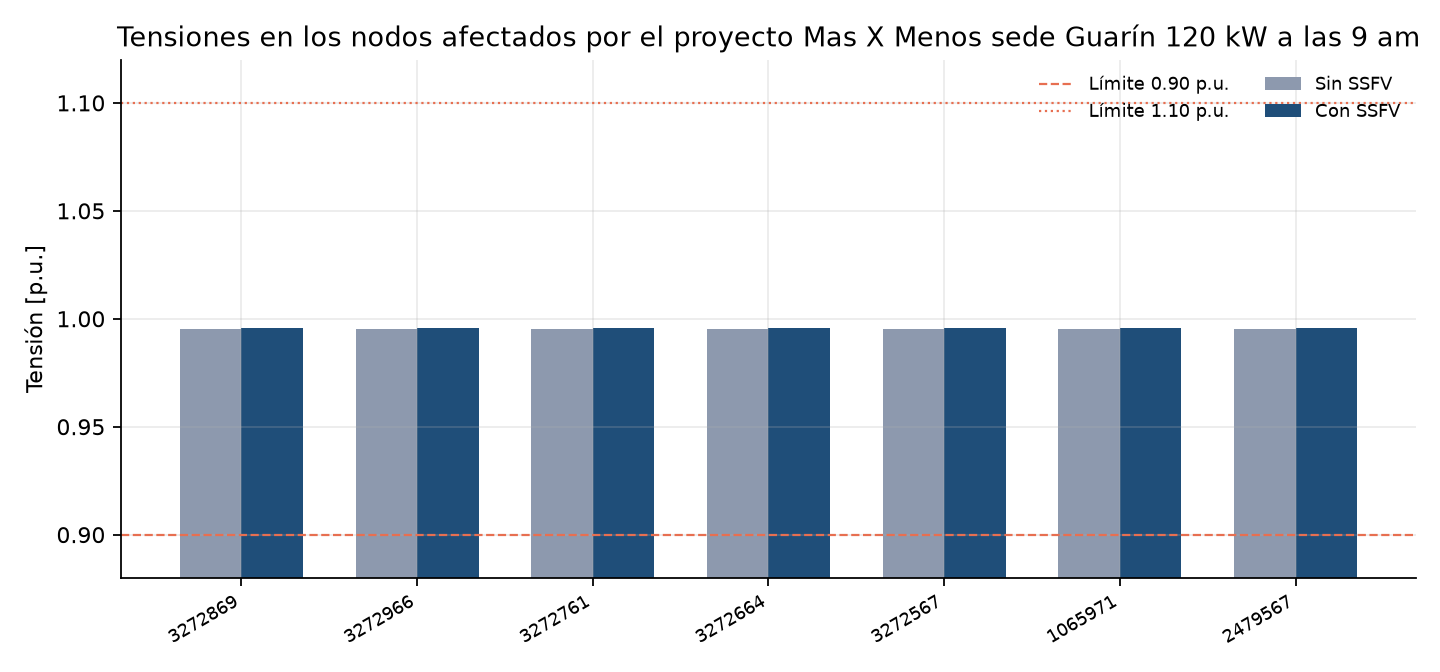
\includegraphics[width=\textwidth]{figuras/fig_tensiones_09.png}
    \caption{Tensiones en los nodos afectados por el proyecto Mas X Menos sede Guarín 120~kW a las 9~am}
    \label{fig:tensiones9}
\end{figure}

\begin{figure}[H]
    \centering
    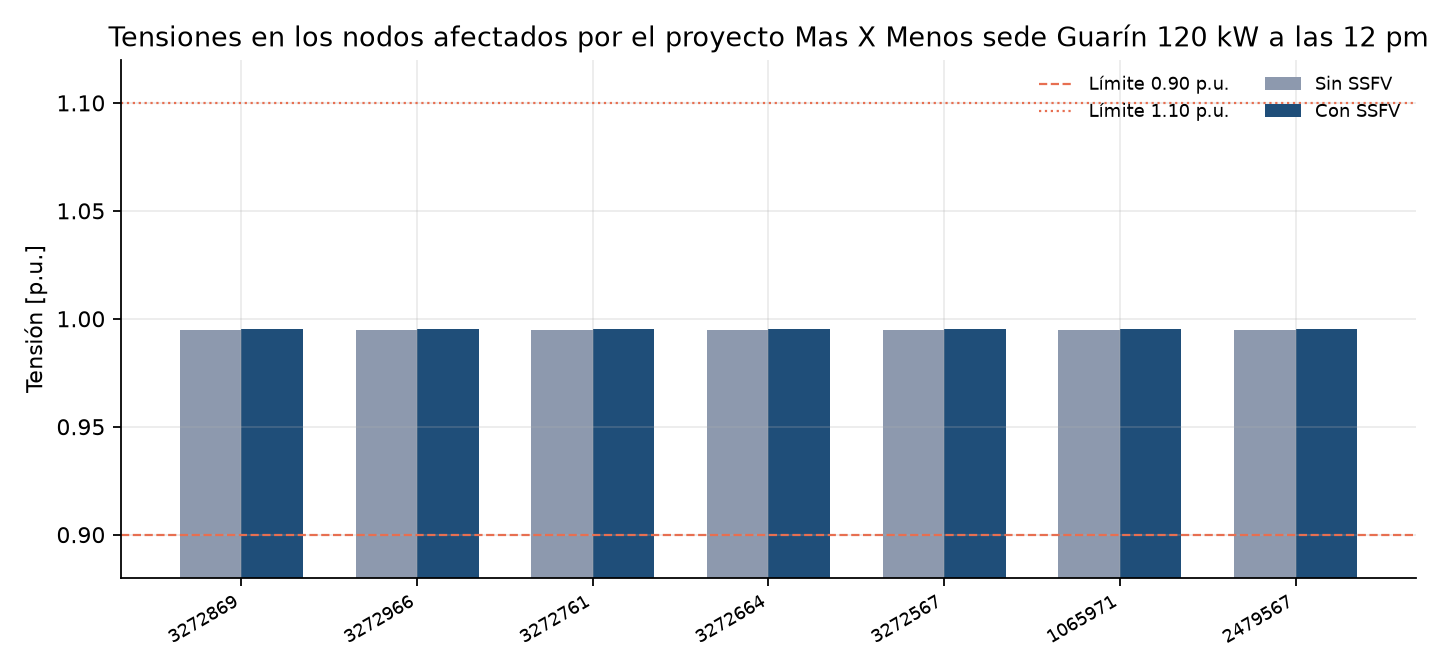
\includegraphics[width=\textwidth]{figuras/fig_tensiones_12.png}
    \caption{Tensiones en los nodos afectados por el proyecto Mas X Menos sede Guarín 120~kW a las 12~pm}
    \label{fig:tensiones}
\end{figure}

\begin{figure}[H]
    \centering
    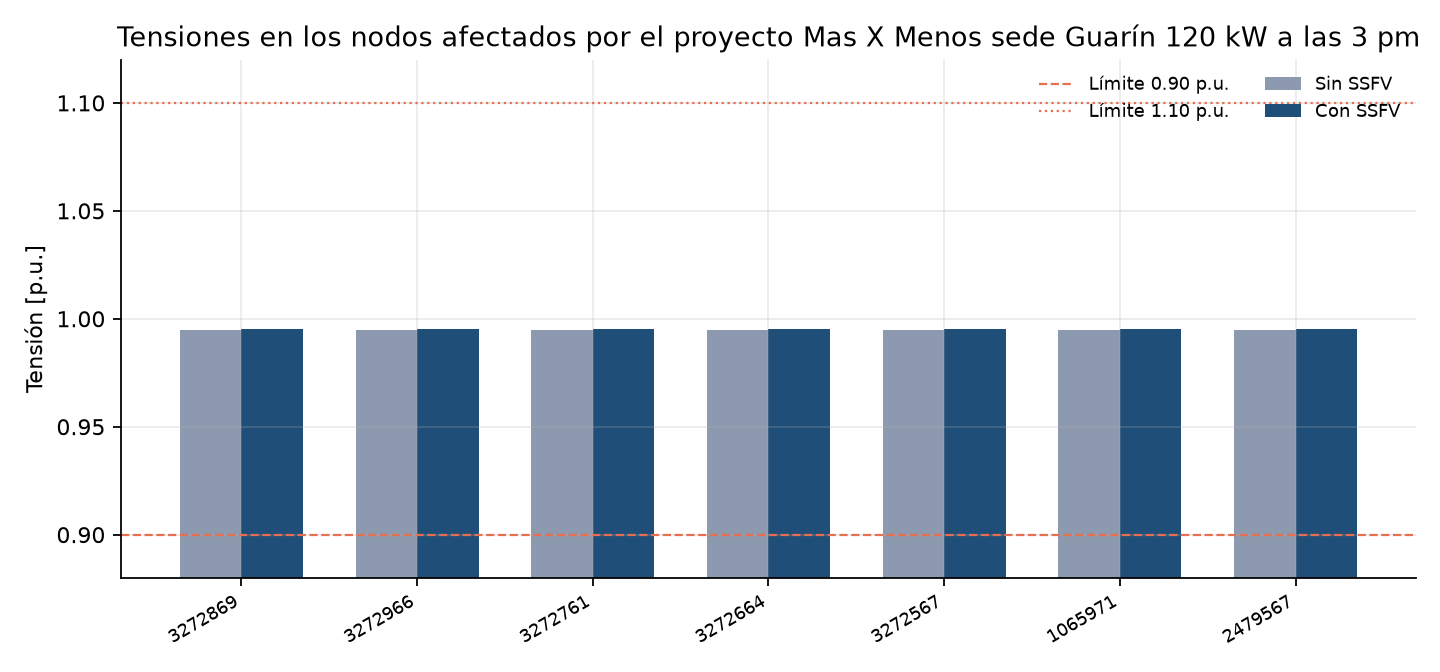
\includegraphics[width=\textwidth]{figuras/fig_tensiones_15.png}
    \caption{Tensiones en los nodos afectados por el proyecto Mas X Menos sede Guarín 120~kW a las 3~pm}
    \label{fig:tensiones15}
\end{figure}

\begin{table}[H]
    \centering
    \caption{Variación de tensión a las 9:00 a.m.}
    \label{tab:v_9}
    \begin{tabular}{lccc}
\toprule
\textbf{Nodo} & \textbf{Sin SSFV (p.u.)} & \textbf{Con SSFV (p.u.)} & \textbf{Variación (p.u.)} \\
\midrule
3272869 & 0,995305 & 0,995918 & 0,000613 \\
3272966 & 0,995304 & 0,995918 & 0,000614 \\
3272761 & 0,995306 & 0,995917 & 0,000611 \\
3272664 & 0,995308 & 0,995916 & 0,000608 \\
3272567 & 0,995314 & 0,995914 & 0,000600 \\
1065971 & 0,995312 & 0,995908 & 0,000596 \\
2479567 & 0,995312 & 0,995908 & 0,000596 \\
\bottomrule
\end{tabular}

\end{table}

\begin{table}[H]
    \centering
    \caption{Variación de tensión a las 12:00 p.m.}
    \label{tab:v_12}
    \begin{tabular}{lccc}
\toprule
\textbf{Nodo} & \textbf{Sin SSFV (p.u.)} & \textbf{Con SSFV (p.u.)} & \textbf{Variación (p.u.)} \\
\midrule
3272869 & 0,994584 & 0,995201 & 0,000617 \\
3272966 & 0,994583 & 0,995201 & 0,000618 \\
3272761 & 0,994586 & 0,995201 & 0,000615 \\
3272664 & 0,994588 & 0,995200 & 0,000612 \\
3272567 & 0,994594 & 0,995199 & 0,000605 \\
1065971 & 0,994592 & 0,995192 & 0,000600 \\
2479567 & 0,994592 & 0,995192 & 0,000600 \\
\bottomrule
\end{tabular}

\end{table}

\begin{table}[H]
    \centering
    \caption{Variación de tensión a las 15:00}
    \label{tab:v_15}
    \begin{tabular}{lccc}
\toprule
\textbf{Nodo} & \textbf{Sin SSFV (p.u.)} & \textbf{Con SSFV (p.u.)} & \textbf{Variación (p.u.)} \\
\midrule
3272869 & 0,994743 & 0,995350 & 0,000607 \\
3272966 & 0,994742 & 0,995350 & 0,000608 \\
3272761 & 0,994745 & 0,995350 & 0,000605 \\
3272664 & 0,994747 & 0,995349 & 0,000602 \\
3272567 & 0,994753 & 0,995347 & 0,000594 \\
1065971 & 0,994755 & 0,995344 & 0,000589 \\
2479567 & 0,994755 & 0,995344 & 0,000589 \\
\bottomrule
\end{tabular}

\end{table}

En las tres franjas evaluadas las tensiones permanecen dentro de la banda 0,90--1,10~p.u. en \textbf{todos} los nodos energizados. El efecto del SSFV es una leve elevación local de tensión, compatible con el Código de Redes. Las Tablas~\ref{tab:v_todas_09}, \ref{tab:v_todas_12} y~\ref{tab:v_todas_15} listan las 181--185 barras del modelo (sin y con SSFV).

\begingroup
\footnotesize
\setlength{\tabcolsep}{3.5pt}
\begin{longtable}{lccccc}
\caption{Tensiones en todos los nodos energizados a las 9:00 a.m. (sin y con SSFV)} \label{tab:v_todas_09} \\
\toprule
\textbf{Nodo} & \textbf{$U_n$ (kV)} & \textbf{Sin SSFV (p.u.)} & \textbf{Con SSFV (p.u.)} & \textbf{$\Delta U$ (p.u.)} & \textbf{Banda} \\
\midrule
\endfirsthead
\caption[]{Tensiones en todos los nodos energizados a las 9:00 a.m. (sin y con SSFV) (cont.)} \\
\toprule
\textbf{Nodo} & \textbf{$U_n$ (kV)} & \textbf{Sin SSFV (p.u.)} & \textbf{Con SSFV (p.u.)} & \textbf{$\Delta U$ (p.u.)} & \textbf{Banda} \\
\midrule
\endhead
\midrule
\multicolumn{6}{r}{\textit{Continúa en la página siguiente}} \\
\endfoot
\bottomrule
\endlastfoot
10 502\_Term & 13,8 & 1,000000 & 1,000000 & 0,000000 & Sí \\
1067001 & 13,8 & 0,999983 & 0,999984 & 0,000001 & Sí \\
3272966 & 13,8 & 0,995304 & 0,995918 & 0,000614 & Sí \\
220 V & 0,2 & 0,982301 & 0,993503 & 0,011202 & Sí \\
1026666 & 13,8 & 0,997557 & 0,997685 & 0,000128 & Sí \\
1026682 & 13,8 & 0,997557 & 0,997686 & 0,000129 & Sí \\
1045288 & 13,8 & 0,995664 & 0,996098 & 0,000434 & Sí \\
1065971 & 13,8 & 0,995312 & 0,995908 & 0,000596 & Sí \\
1067010 & 13,8 & 0,998198 & 0,998289 & 0,000091 & Sí \\
1067028 & 13,8 & 0,998039 & 0,998138 & 0,000099 & Sí \\
1067036 & 13,8 & 0,998007 & 0,998109 & 0,000102 & Sí \\
1067044 & 13,8 & 0,997872 & 0,997981 & 0,000109 & Sí \\
1067052 & 13,8 & 0,997726 & 0,997844 & 0,000118 & Sí \\
1067079 & 13,8 & 0,997719 & 0,997838 & 0,000119 & Sí \\
1067087 & 13,8 & 0,997715 & 0,997833 & 0,000118 & Sí \\
1067109 & 13,8 & 0,997576 & 0,997705 & 0,000129 & Sí \\
1067117 & 13,8 & 0,997382 & 0,997528 & 0,000146 & Sí \\
1067125 & 13,8 & 0,997218 & 0,997380 & 0,000162 & Sí \\
1067133 & 13,8 & 0,997216 & 0,997377 & 0,000161 & Sí \\
1067141 & 13,8 & 0,997088 & 0,997262 & 0,000174 & Sí \\
1067150 & 13,8 & 0,996899 & 0,997094 & 0,000195 & Sí \\
1067176 & 13,8 & 0,996712 & 0,996926 & 0,000214 & Sí \\
1067184 & 13,8 & 0,996630 & 0,996855 & 0,000225 & Sí \\
1067192 & 13,8 & 0,996524 & 0,996764 & 0,000240 & Sí \\
1067206 & 13,8 & 0,996414 & 0,996670 & 0,000256 & Sí \\
1067214 & 13,8 & 0,996305 & 0,996579 & 0,000274 & Sí \\
1069438 & 13,8 & 0,999846 & 0,999854 & 0,000008 & Sí \\
1069446 & 13,8 & 0,999529 & 0,999552 & 0,000023 & Sí \\
1069454 & 13,8 & 0,999449 & 0,999477 & 0,000028 & Sí \\
1069471 & 13,8 & 0,999319 & 0,999354 & 0,000035 & Sí \\
1069489 & 13,8 & 0,999092 & 0,999138 & 0,000046 & Sí \\
1069497 & 13,8 & 0,998897 & 0,998952 & 0,000055 & Sí \\
1069501 & 13,8 & 0,998722 & 0,998786 & 0,000064 & Sí \\
1069519 & 13,8 & 0,998582 & 0,998653 & 0,000071 & Sí \\
1069527 & 13,8 & 0,998530 & 0,998604 & 0,000074 & Sí \\
1069683 & 13,8 & 0,998301 & 0,998386 & 0,000085 & Sí \\
1101251 & 13,8 & 0,996262 & 0,996543 & 0,000281 & Sí \\
1101277 & 13,8 & 0,996203 & 0,996495 & 0,000292 & Sí \\
1101293 & 13,8 & 0,995985 & 0,996316 & 0,000331 & Sí \\
1101307 & 13,8 & 0,995906 & 0,996255 & 0,000349 & Sí \\
1101315 & 13,8 & 0,995832 & 0,996203 & 0,000371 & Sí \\
1101323 & 13,8 & 0,995781 & 0,996171 & 0,000390 & Sí \\
1101331 & 13,8 & 0,995734 & 0,996142 & 0,000408 & Sí \\
1101340 & 13,8 & 0,995674 & 0,996104 & 0,000430 & Sí \\
1101358 & 13,8 & 0,995636 & 0,996082 & 0,000446 & Sí \\
1101374 & 13,8 & 0,995579 & 0,996049 & 0,000470 & Sí \\
1101382 & 13,8 & 0,995536 & 0,996024 & 0,000488 & Sí \\
1101391 & 13,8 & 0,995496 & 0,996001 & 0,000505 & Sí \\
1101404 & 13,8 & 0,995430 & 0,995963 & 0,000533 & Sí \\
1101412 & 13,8 & 0,995394 & 0,995944 & 0,000550 & Sí \\
1101421 & 13,8 & 0,995360 & 0,995927 & 0,000567 & Sí \\
1101447 & 13,8 & 0,995341 & 0,995920 & 0,000579 & Sí \\
1101455 & 13,8 & 0,995317 & 0,995913 & 0,000596 & Sí \\
1101471 & 13,8 & 0,995312 & 0,995908 & 0,000596 & Sí \\
1101480 & 13,8 & 0,995312 & 0,995908 & 0,000596 & Sí \\
1102958 & 13,8 & 0,997574 & 0,997703 & 0,000129 & Sí \\
1102974 & 13,8 & 0,997571 & 0,997700 & 0,000129 & Sí \\
1102982 & 13,8 & 0,997558 & 0,997686 & 0,000128 & Sí \\
1103211 & 13,8 & 0,996626 & 0,996851 & 0,000225 & Sí \\
1103229 & 13,8 & 0,996626 & 0,996850 & 0,000224 & Sí \\
1103245 & 13,8 & 0,996523 & 0,996763 & 0,000240 & Sí \\
1103253 & 13,8 & 0,996520 & 0,996760 & 0,000240 & Sí \\
1103296 & 13,8 & 0,997215 & 0,997376 & 0,000161 & Sí \\
1103300 & 13,8 & 0,997215 & 0,997376 & 0,000161 & Sí \\
1103318 & 13,8 & 0,997214 & 0,997376 & 0,000162 & Sí \\
1103326 & 13,8 & 0,997214 & 0,997376 & 0,000162 & Sí \\
1103351 & 13,8 & 0,996524 & 0,996763 & 0,000239 & Sí \\
1103385 & 13,8 & 0,996523 & 0,996763 & 0,000240 & Sí \\
1103393 & 13,8 & 0,996412 & 0,996669 & 0,000257 & Sí \\
1103407 & 13,8 & 0,996409 & 0,996665 & 0,000256 & Sí \\
1103431 & 13,8 & 0,996203 & 0,996494 & 0,000291 & Sí \\
1103458 & 13,8 & 0,996201 & 0,996492 & 0,000291 & Sí \\
1103725 & 13,8 & 0,996304 & 0,996578 & 0,000274 & Sí \\
1154079 & 13,8 & 0,998197 & 0,998288 & 0,000091 & Sí \\
1154087 & 13,8 & 0,998190 & 0,998281 & 0,000091 & Sí \\
1154109 & 13,8 & 0,998191 & 0,998281 & 0,000090 & Sí \\
1154117 & 13,8 & 0,998193 & 0,998283 & 0,000090 & Sí \\
1154125 & 13,8 & 0,998194 & 0,998284 & 0,000090 & Sí \\
1154133 & 13,8 & 0,998037 & 0,998137 & 0,000100 & Sí \\
1154141 & 13,8 & 0,998038 & 0,998138 & 0,000100 & Sí \\
1154150 & 13,8 & 0,998037 & 0,998137 & 0,000100 & Sí \\
1154176 & 13,8 & 0,998036 & 0,998136 & 0,000100 & Sí \\
1154192 & 13,8 & 0,998005 & 0,998107 & 0,000102 & Sí \\
1154206 & 13,8 & 0,998006 & 0,998108 & 0,000102 & Sí \\
1154214 & 13,8 & 0,996666 & 0,996880 & 0,000214 & Sí \\
1154222 & 13,8 & 0,998004 & 0,998106 & 0,000102 & Sí \\
1154231 & 13,8 & 0,998001 & 0,998102 & 0,000101 & Sí \\
1154249 & 13,8 & 0,997087 & 0,997261 & 0,000174 & Sí \\
1154257 & 13,8 & 0,997086 & 0,997260 & 0,000174 & Sí \\
1154273 & 13,8 & 0,997085 & 0,997259 & 0,000174 & Sí \\
1154281 & 13,8 & 0,997083 & 0,997258 & 0,000175 & Sí \\
1154290 & 13,8 & 0,997084 & 0,997258 & 0,000174 & Sí \\
1154303 & 13,8 & 0,998037 & 0,998137 & 0,000100 & Sí \\
1154311 & 13,8 & 0,997378 & 0,997524 & 0,000146 & Sí \\
1154346 & 13,8 & 0,997381 & 0,997527 & 0,000146 & Sí \\
1154354 & 13,8 & 0,997380 & 0,997526 & 0,000146 & Sí \\
1154371 & 13,8 & 0,996707 & 0,996921 & 0,000214 & Sí \\
1154389 & 13,8 & 0,996707 & 0,996921 & 0,000214 & Sí \\
1154397 & 13,8 & 0,996694 & 0,996908 & 0,000214 & Sí \\
1154401 & 13,8 & 0,996675 & 0,996889 & 0,000214 & Sí \\
1154435 & 13,8 & 0,998000 & 0,998102 & 0,000102 & Sí \\
1154443 & 13,8 & 0,997218 & 0,997379 & 0,000161 & Sí \\
1154451 & 13,8 & 0,997217 & 0,997378 & 0,000161 & Sí \\
1154478 & 13,8 & 0,997216 & 0,997377 & 0,000161 & Sí \\
1154494 & 13,8 & 0,997214 & 0,997376 & 0,000162 & Sí \\
1154508 & 13,8 & 0,997558 & 0,997687 & 0,000129 & Sí \\
1154524 & 13,8 & 0,996629 & 0,996854 & 0,000225 & Sí \\
1154532 & 13,8 & 0,996626 & 0,996851 & 0,000225 & Sí \\
1154541 & 13,8 & 0,996624 & 0,996849 & 0,000225 & Sí \\
1154575 & 13,8 & 0,996629 & 0,996854 & 0,000225 & Sí \\
1154583 & 13,8 & 0,996626 & 0,996851 & 0,000225 & Sí \\
1154591 & 13,8 & 0,996624 & 0,996848 & 0,000224 & Sí \\
1154605 & 13,8 & 0,996303 & 0,996577 & 0,000274 & Sí \\
1154613 & 13,8 & 0,996303 & 0,996577 & 0,000274 & Sí \\
1155245 & 13,8 & 0,995979 & 0,996310 & 0,000331 & Sí \\
1155253 & 13,8 & 0,995972 & 0,996302 & 0,000330 & Sí \\
1155270 & 13,8 & 0,995974 & 0,996305 & 0,000331 & Sí \\
1155334 & 13,8 & 0,995830 & 0,996202 & 0,000372 & Sí \\
1155342 & 13,8 & 0,995829 & 0,996200 & 0,000371 & Sí \\
1155351 & 13,8 & 0,995827 & 0,996199 & 0,000372 & Sí \\
1155377 & 13,8 & 0,995825 & 0,996197 & 0,000372 & Sí \\
1155652 & 13,8 & 0,995673 & 0,996103 & 0,000430 & Sí \\
1155679 & 13,8 & 0,995825 & 0,996196 & 0,000371 & Sí \\
1155741 & 13,8 & 0,995359 & 0,995926 & 0,000567 & Sí \\
1155750 & 13,8 & 0,995357 & 0,995924 & 0,000567 & Sí \\
1155776 & 13,8 & 0,995357 & 0,995923 & 0,000566 & Sí \\
1155792 & 13,8 & 0,995358 & 0,995925 & 0,000567 & Sí \\
1155806 & 13,8 & 0,995356 & 0,995922 & 0,000566 & Sí \\
1155822 & 13,8 & 0,995355 & 0,995922 & 0,000567 & Sí \\
1155849 & 13,8 & 0,995429 & 0,995962 & 0,000533 & Sí \\
1155857 & 13,8 & 0,995428 & 0,995961 & 0,000533 & Sí \\
1155881 & 13,8 & 0,995428 & 0,995960 & 0,000532 & Sí \\
1155911 & 13,8 & 0,995971 & 0,996301 & 0,000330 & Sí \\
1155938 & 13,8 & 0,995673 & 0,996103 & 0,000430 & Sí \\
1155946 & 13,8 & 0,995671 & 0,996101 & 0,000430 & Sí \\
1155971 & 13,8 & 0,995672 & 0,996102 & 0,000430 & Sí \\
1155997 & 13,8 & 0,995672 & 0,996102 & 0,000430 & Sí \\
1157019 & 13,8 & 0,995829 & 0,996200 & 0,000371 & Sí \\
1283235 & 13,8 & 0,997709 & 0,997828 & 0,000119 & Sí \\
1618733 & 13,8 & 0,995427 & 0,995959 & 0,000532 & Sí \\
1618741 & 13,8 & 0,995429 & 0,995962 & 0,000533 & Sí \\
1618750 & 13,8 & 0,995429 & 0,995962 & 0,000533 & Sí \\
1667238 & 13,8 & 0,996304 & 0,996578 & 0,000274 & Sí \\
1667262 & 13,8 & 0,996409 & 0,996666 & 0,000257 & Sí \\
2214130 & 13,8 & 0,995904 & 0,996254 & 0,000350 & Sí \\
2214148 & 13,8 & 0,995902 & 0,996251 & 0,000349 & Sí \\
2214156 & 13,8 & 0,995901 & 0,996251 & 0,000350 & Sí \\
2479567 & 13,8 & 0,995312 & 0,995908 & 0,000596 & Sí \\
2567814 & 13,8 & 0,995971 & 0,996302 & 0,000331 & Sí \\
2567831 & 13,8 & 0,995971 & 0,996301 & 0,000330 & Sí \\
2765811 & 13,8 & 0,998191 & 0,998281 & 0,000090 & Sí \\
2765829 & 13,8 & 0,998177 & 0,998268 & 0,000091 & Sí \\
2765837 & 13,8 & 0,998176 & 0,998266 & 0,000090 & Sí \\
2789132 & 13,8 & 0,995356 & 0,995923 & 0,000567 & Sí \\
2789141 & 13,8 & 0,995356 & 0,995922 & 0,000566 & Sí \\
3272567 & 13,8 & 0,995314 & 0,995914 & 0,000600 & Sí \\
3272664 & 13,8 & 0,995308 & 0,995916 & 0,000608 & Sí \\
3272761 & 13,8 & 0,995306 & 0,995917 & 0,000611 & Sí \\
3272869 & 13,8 & 0,995305 & 0,995918 & 0,000613 & Sí \\
3453260 & 13,8 & 0,995963 & 0,996293 & 0,000330 & Sí \\
3453367 & 13,8 & 0,995964 & 0,996294 & 0,000330 & Sí \\
3453464 & 13,8 & 0,995966 & 0,996296 & 0,000330 & Sí \\
3453561 & 13,8 & 0,995971 & 0,996301 & 0,000330 & Sí \\
3769721 & 13,8 & 0,996108 & 0,996417 & 0,000309 & Sí \\
4249330 & 13,8 & 0,997712 & 0,997830 & 0,000118 & Sí \\
4249348 & 13,8 & 0,997710 & 0,997828 & 0,000118 & Sí \\
4249356 & 13,8 & 0,997706 & 0,997824 & 0,000118 & Sí \\
4249372 & 13,8 & 0,997705 & 0,997823 & 0,000118 & Sí \\
4938216 & 13,8 & 0,995901 & 0,996251 & 0,000350 & Sí \\
5604524 & 13,8 & 0,997709 & 0,997827 & 0,000118 & Sí \\
5605024 & 13,8 & 0,997717 & 0,997835 & 0,000118 & Sí \\
5605032 & 13,8 & 0,997715 & 0,997833 & 0,000118 & Sí \\
8338973 & 13,8 & 0,997555 & 0,997684 & 0,000129 & Sí \\
8339155 & 13,8 & 0,997556 & 0,997684 & 0,000128 & Sí \\
8339694 & 13,8 & 0,997555 & 0,997684 & 0,000129 & Sí \\
8339708 & 13,8 & 0,997557 & 0,997686 & 0,000129 & Sí \\
8795266 & 13,8 & 0,997720 & 0,997839 & 0,000119 & Sí \\
9219013 & 13,8 & 0,995426 & 0,995959 & 0,000533 & Sí \\
9500758 & 13,8 & 0,997725 & 0,997843 & 0,000118 & Sí \\
9500766 & 13,8 & 0,997723 & 0,997841 & 0,000118 & Sí \\
9500774 & 13,8 & 0,997721 & 0,997839 & 0,000118 & Sí \\
\end{longtable}
\endgroup

\begingroup
\footnotesize
\setlength{\tabcolsep}{3.5pt}
\begin{longtable}{lccccc}
\caption{Tensiones en todos los nodos energizados a las 12:00 p.m. (sin y con SSFV)} \label{tab:v_todas_12} \\
\toprule
\textbf{Nodo} & \textbf{$U_n$ (kV)} & \textbf{Sin SSFV (p.u.)} & \textbf{Con SSFV (p.u.)} & \textbf{$\Delta U$ (p.u.)} & \textbf{Banda} \\
\midrule
\endfirsthead
\caption[]{Tensiones en todos los nodos energizados a las 12:00 p.m. (sin y con SSFV) (cont.)} \\
\toprule
\textbf{Nodo} & \textbf{$U_n$ (kV)} & \textbf{Sin SSFV (p.u.)} & \textbf{Con SSFV (p.u.)} & \textbf{$\Delta U$ (p.u.)} & \textbf{Banda} \\
\midrule
\endhead
\midrule
\multicolumn{6}{r}{\textit{Continúa en la página siguiente}} \\
\endfoot
\bottomrule
\endlastfoot
10 502\_Term & 13,8 & 1,000000 & 1,000000 & 0,000000 & Sí \\
1067001 & 13,8 & 0,999980 & 0,999981 & 0,000001 & Sí \\
3272966 & 13,8 & 0,994583 & 0,995201 & 0,000618 & Sí \\
220 V & 0,2 & 0,980435 & 0,991736 & 0,011301 & Sí \\
1026666 & 13,8 & 0,997181 & 0,997311 & 0,000130 & Sí \\
1026682 & 13,8 & 0,997181 & 0,997311 & 0,000130 & Sí \\
1045288 & 13,8 & 0,994998 & 0,995435 & 0,000437 & Sí \\
1065971 & 13,8 & 0,994592 & 0,995192 & 0,000600 & Sí \\
1067010 & 13,8 & 0,997921 & 0,998013 & 0,000092 & Sí \\
1067028 & 13,8 & 0,997737 & 0,997838 & 0,000101 & Sí \\
1067036 & 13,8 & 0,997701 & 0,997803 & 0,000102 & Sí \\
1067044 & 13,8 & 0,997544 & 0,997655 & 0,000111 & Sí \\
1067052 & 13,8 & 0,997376 & 0,997496 & 0,000120 & Sí \\
1067079 & 13,8 & 0,997369 & 0,997488 & 0,000119 & Sí \\
1067087 & 13,8 & 0,997364 & 0,997483 & 0,000119 & Sí \\
1067109 & 13,8 & 0,997203 & 0,997333 & 0,000130 & Sí \\
1067117 & 13,8 & 0,996979 & 0,997127 & 0,000148 & Sí \\
1067125 & 13,8 & 0,996791 & 0,996953 & 0,000162 & Sí \\
1067133 & 13,8 & 0,996788 & 0,996950 & 0,000162 & Sí \\
1067141 & 13,8 & 0,996640 & 0,996816 & 0,000176 & Sí \\
1067150 & 13,8 & 0,996422 & 0,996619 & 0,000197 & Sí \\
1067176 & 13,8 & 0,996206 & 0,996422 & 0,000216 & Sí \\
1067184 & 13,8 & 0,996112 & 0,996338 & 0,000226 & Sí \\
1067192 & 13,8 & 0,995990 & 0,996232 & 0,000242 & Sí \\
1067206 & 13,8 & 0,995863 & 0,996121 & 0,000258 & Sí \\
1067214 & 13,8 & 0,995737 & 0,996013 & 0,000276 & Sí \\
1069438 & 13,8 & 0,999822 & 0,999830 & 0,000008 & Sí \\
1069446 & 13,8 & 0,999456 & 0,999480 & 0,000024 & Sí \\
1069454 & 13,8 & 0,999364 & 0,999392 & 0,000028 & Sí \\
1069471 & 13,8 & 0,999215 & 0,999249 & 0,000034 & Sí \\
1069489 & 13,8 & 0,998953 & 0,998999 & 0,000046 & Sí \\
1069497 & 13,8 & 0,998727 & 0,998783 & 0,000056 & Sí \\
1069501 & 13,8 & 0,998526 & 0,998591 & 0,000065 & Sí \\
1069519 & 13,8 & 0,998364 & 0,998436 & 0,000072 & Sí \\
1069527 & 13,8 & 0,998304 & 0,998379 & 0,000075 & Sí \\
1069683 & 13,8 & 0,998039 & 0,998126 & 0,000087 & Sí \\
1101251 & 13,8 & 0,995687 & 0,995970 & 0,000283 & Sí \\
1101277 & 13,8 & 0,995620 & 0,995913 & 0,000293 & Sí \\
1101293 & 13,8 & 0,995368 & 0,995701 & 0,000333 & Sí \\
1101307 & 13,8 & 0,995277 & 0,995629 & 0,000352 & Sí \\
1101315 & 13,8 & 0,995191 & 0,995565 & 0,000374 & Sí \\
1101323 & 13,8 & 0,995132 & 0,995525 & 0,000393 & Sí \\
1101331 & 13,8 & 0,995079 & 0,995489 & 0,000410 & Sí \\
1101340 & 13,8 & 0,995009 & 0,995442 & 0,000433 & Sí \\
1101358 & 13,8 & 0,994965 & 0,995414 & 0,000449 & Sí \\
1101374 & 13,8 & 0,994900 & 0,995373 & 0,000473 & Sí \\
1101382 & 13,8 & 0,994850 & 0,995341 & 0,000491 & Sí \\
1101391 & 13,8 & 0,994804 & 0,995312 & 0,000508 & Sí \\
1101404 & 13,8 & 0,994728 & 0,995264 & 0,000536 & Sí \\
1101412 & 13,8 & 0,994687 & 0,995240 & 0,000553 & Sí \\
1101421 & 13,8 & 0,994648 & 0,995218 & 0,000570 & Sí \\
1101447 & 13,8 & 0,994626 & 0,995209 & 0,000583 & Sí \\
1101455 & 13,8 & 0,994598 & 0,995198 & 0,000600 & Sí \\
1101471 & 13,8 & 0,994592 & 0,995192 & 0,000600 & Sí \\
1101480 & 13,8 & 0,994592 & 0,995192 & 0,000600 & Sí \\
1102958 & 13,8 & 0,997201 & 0,997331 & 0,000130 & Sí \\
1102974 & 13,8 & 0,997198 & 0,997328 & 0,000130 & Sí \\
1102982 & 13,8 & 0,997182 & 0,997312 & 0,000130 & Sí \\
1103211 & 13,8 & 0,996107 & 0,996334 & 0,000227 & Sí \\
1103229 & 13,8 & 0,996107 & 0,996333 & 0,000226 & Sí \\
1103245 & 13,8 & 0,995989 & 0,996230 & 0,000241 & Sí \\
1103253 & 13,8 & 0,995985 & 0,996227 & 0,000242 & Sí \\
1103296 & 13,8 & 0,996787 & 0,996950 & 0,000163 & Sí \\
1103300 & 13,8 & 0,996787 & 0,996949 & 0,000162 & Sí \\
1103318 & 13,8 & 0,996786 & 0,996949 & 0,000163 & Sí \\
1103326 & 13,8 & 0,996786 & 0,996949 & 0,000163 & Sí \\
1103351 & 13,8 & 0,995989 & 0,996231 & 0,000242 & Sí \\
1103385 & 13,8 & 0,995988 & 0,996230 & 0,000242 & Sí \\
1103393 & 13,8 & 0,995861 & 0,996119 & 0,000258 & Sí \\
1103407 & 13,8 & 0,995857 & 0,996115 & 0,000258 & Sí \\
1103431 & 13,8 & 0,995619 & 0,995912 & 0,000293 & Sí \\
1103458 & 13,8 & 0,995617 & 0,995910 & 0,000293 & Sí \\
1103725 & 13,8 & 0,995736 & 0,996012 & 0,000276 & Sí \\
1154079 & 13,8 & 0,997920 & 0,998011 & 0,000091 & Sí \\
1154087 & 13,8 & 0,997912 & 0,998003 & 0,000091 & Sí \\
1154109 & 13,8 & 0,997913 & 0,998004 & 0,000091 & Sí \\
1154117 & 13,8 & 0,997915 & 0,998006 & 0,000091 & Sí \\
1154125 & 13,8 & 0,997916 & 0,998008 & 0,000092 & Sí \\
1154133 & 13,8 & 0,997735 & 0,997836 & 0,000101 & Sí \\
1154141 & 13,8 & 0,997736 & 0,997837 & 0,000101 & Sí \\
1154150 & 13,8 & 0,997735 & 0,997836 & 0,000101 & Sí \\
1154176 & 13,8 & 0,997734 & 0,997835 & 0,000101 & Sí \\
1154192 & 13,8 & 0,997698 & 0,997801 & 0,000103 & Sí \\
1154206 & 13,8 & 0,997700 & 0,997802 & 0,000102 & Sí \\
1154214 & 13,8 & 0,996153 & 0,996369 & 0,000216 & Sí \\
1154222 & 13,8 & 0,997698 & 0,997800 & 0,000102 & Sí \\
1154231 & 13,8 & 0,997693 & 0,997795 & 0,000102 & Sí \\
1154249 & 13,8 & 0,996639 & 0,996814 & 0,000175 & Sí \\
1154257 & 13,8 & 0,996638 & 0,996814 & 0,000176 & Sí \\
1154273 & 13,8 & 0,996637 & 0,996812 & 0,000175 & Sí \\
1154281 & 13,8 & 0,996635 & 0,996811 & 0,000176 & Sí \\
1154290 & 13,8 & 0,996635 & 0,996811 & 0,000176 & Sí \\
1154303 & 13,8 & 0,997735 & 0,997836 & 0,000101 & Sí \\
1154311 & 13,8 & 0,996975 & 0,997122 & 0,000147 & Sí \\
1154346 & 13,8 & 0,996978 & 0,997126 & 0,000148 & Sí \\
1154354 & 13,8 & 0,996977 & 0,997125 & 0,000148 & Sí \\
1154371 & 13,8 & 0,996201 & 0,996416 & 0,000215 & Sí \\
1154389 & 13,8 & 0,996201 & 0,996417 & 0,000216 & Sí \\
1154397 & 13,8 & 0,996186 & 0,996401 & 0,000215 & Sí \\
1154401 & 13,8 & 0,996164 & 0,996379 & 0,000215 & Sí \\
1154435 & 13,8 & 0,997693 & 0,997795 & 0,000102 & Sí \\
1154443 & 13,8 & 0,996790 & 0,996952 & 0,000162 & Sí \\
1154451 & 13,8 & 0,996789 & 0,996952 & 0,000163 & Sí \\
1154478 & 13,8 & 0,996788 & 0,996950 & 0,000162 & Sí \\
1154494 & 13,8 & 0,996786 & 0,996949 & 0,000163 & Sí \\
1154508 & 13,8 & 0,997182 & 0,997312 & 0,000130 & Sí \\
1154524 & 13,8 & 0,996111 & 0,996337 & 0,000226 & Sí \\
1154532 & 13,8 & 0,996107 & 0,996334 & 0,000227 & Sí \\
1154541 & 13,8 & 0,996105 & 0,996332 & 0,000227 & Sí \\
1154575 & 13,8 & 0,996111 & 0,996337 & 0,000226 & Sí \\
1154583 & 13,8 & 0,996108 & 0,996334 & 0,000226 & Sí \\
1154591 & 13,8 & 0,996105 & 0,996331 & 0,000226 & Sí \\
1154605 & 13,8 & 0,995735 & 0,996011 & 0,000276 & Sí \\
1154613 & 13,8 & 0,995735 & 0,996011 & 0,000276 & Sí \\
1155245 & 13,8 & 0,995362 & 0,995695 & 0,000333 & Sí \\
1155253 & 13,8 & 0,995353 & 0,995686 & 0,000333 & Sí \\
1155270 & 13,8 & 0,995356 & 0,995689 & 0,000333 & Sí \\
1155334 & 13,8 & 0,995190 & 0,995564 & 0,000374 & Sí \\
1155342 & 13,8 & 0,995188 & 0,995562 & 0,000374 & Sí \\
1155351 & 13,8 & 0,995186 & 0,995560 & 0,000374 & Sí \\
1155377 & 13,8 & 0,995184 & 0,995558 & 0,000374 & Sí \\
1155652 & 13,8 & 0,995008 & 0,995441 & 0,000433 & Sí \\
1155679 & 13,8 & 0,995183 & 0,995557 & 0,000374 & Sí \\
1155741 & 13,8 & 0,994647 & 0,995217 & 0,000570 & Sí \\
1155750 & 13,8 & 0,994644 & 0,995215 & 0,000571 & Sí \\
1155776 & 13,8 & 0,994644 & 0,995214 & 0,000570 & Sí \\
1155792 & 13,8 & 0,994645 & 0,995216 & 0,000571 & Sí \\
1155806 & 13,8 & 0,994643 & 0,995213 & 0,000570 & Sí \\
1155822 & 13,8 & 0,994642 & 0,995213 & 0,000571 & Sí \\
1155849 & 13,8 & 0,994728 & 0,995264 & 0,000536 & Sí \\
1155857 & 13,8 & 0,994726 & 0,995262 & 0,000536 & Sí \\
1155881 & 13,8 & 0,994725 & 0,995261 & 0,000536 & Sí \\
1155911 & 13,8 & 0,995352 & 0,995685 & 0,000333 & Sí \\
1155938 & 13,8 & 0,995008 & 0,995441 & 0,000433 & Sí \\
1155946 & 13,8 & 0,995006 & 0,995439 & 0,000433 & Sí \\
1155971 & 13,8 & 0,995007 & 0,995440 & 0,000433 & Sí \\
1155997 & 13,8 & 0,995007 & 0,995440 & 0,000433 & Sí \\
1157019 & 13,8 & 0,995188 & 0,995562 & 0,000374 & Sí \\
1283235 & 13,8 & 0,997357 & 0,997477 & 0,000120 & Sí \\
1618733 & 13,8 & 0,994724 & 0,995260 & 0,000536 & Sí \\
1618741 & 13,8 & 0,994727 & 0,995263 & 0,000536 & Sí \\
1618750 & 13,8 & 0,994728 & 0,995264 & 0,000536 & Sí \\
1667238 & 13,8 & 0,995736 & 0,996012 & 0,000276 & Sí \\
1667262 & 13,8 & 0,995857 & 0,996116 & 0,000259 & Sí \\
2214130 & 13,8 & 0,995275 & 0,995627 & 0,000352 & Sí \\
2214148 & 13,8 & 0,995272 & 0,995624 & 0,000352 & Sí \\
2214156 & 13,8 & 0,995271 & 0,995624 & 0,000353 & Sí \\
2479567 & 13,8 & 0,994592 & 0,995192 & 0,000600 & Sí \\
2567814 & 13,8 & 0,995352 & 0,995685 & 0,000333 & Sí \\
2567831 & 13,8 & 0,995352 & 0,995685 & 0,000333 & Sí \\
2765811 & 13,8 & 0,997912 & 0,998004 & 0,000092 & Sí \\
2765829 & 13,8 & 0,997897 & 0,997988 & 0,000091 & Sí \\
2765837 & 13,8 & 0,997895 & 0,997987 & 0,000092 & Sí \\
2789132 & 13,8 & 0,994643 & 0,995213 & 0,000570 & Sí \\
2789141 & 13,8 & 0,994643 & 0,995213 & 0,000570 & Sí \\
3272567 & 13,8 & 0,994594 & 0,995199 & 0,000605 & Sí \\
3272664 & 13,8 & 0,994588 & 0,995200 & 0,000612 & Sí \\
3272761 & 13,8 & 0,994586 & 0,995201 & 0,000615 & Sí \\
3272869 & 13,8 & 0,994584 & 0,995201 & 0,000617 & Sí \\
3453260 & 13,8 & 0,995342 & 0,995675 & 0,000333 & Sí \\
3453367 & 13,8 & 0,995343 & 0,995676 & 0,000333 & Sí \\
3453464 & 13,8 & 0,995346 & 0,995679 & 0,000333 & Sí \\
3453561 & 13,8 & 0,995351 & 0,995685 & 0,000334 & Sí \\
3769721 & 13,8 & 0,995510 & 0,995821 & 0,000311 & Sí \\
4249330 & 13,8 & 0,997360 & 0,997480 & 0,000120 & Sí \\
4249348 & 13,8 & 0,997358 & 0,997477 & 0,000119 & Sí \\
4249356 & 13,8 & 0,997353 & 0,997472 & 0,000119 & Sí \\
4249372 & 13,8 & 0,997352 & 0,997471 & 0,000119 & Sí \\
4938216 & 13,8 & 0,995271 & 0,995624 & 0,000353 & Sí \\
5604524 & 13,8 & 0,997357 & 0,997476 & 0,000119 & Sí \\
5605024 & 13,8 & 0,997366 & 0,997485 & 0,000119 & Sí \\
5605032 & 13,8 & 0,997363 & 0,997482 & 0,000119 & Sí \\
8338973 & 13,8 & 0,997179 & 0,997309 & 0,000130 & Sí \\
8339155 & 13,8 & 0,997180 & 0,997310 & 0,000130 & Sí \\
8339694 & 13,8 & 0,997180 & 0,997309 & 0,000129 & Sí \\
8339708 & 13,8 & 0,997181 & 0,997311 & 0,000130 & Sí \\
8795266 & 13,8 & 0,997370 & 0,997489 & 0,000119 & Sí \\
9219013 & 13,8 & 0,994724 & 0,995260 & 0,000536 & Sí \\
9500758 & 13,8 & 0,997375 & 0,997494 & 0,000119 & Sí \\
9500766 & 13,8 & 0,997373 & 0,997492 & 0,000119 & Sí \\
9500774 & 13,8 & 0,997371 & 0,997490 & 0,000119 & Sí \\
\end{longtable}
\endgroup

\begingroup
\footnotesize
\setlength{\tabcolsep}{3.5pt}
\begin{longtable}{lccccc}
\caption{Tensiones en todos los nodos energizados a las 15:00 (sin y con SSFV)} \label{tab:v_todas_15} \\
\toprule
\textbf{Nodo} & \textbf{$U_n$ (kV)} & \textbf{Sin SSFV (p.u.)} & \textbf{Con SSFV (p.u.)} & \textbf{$\Delta U$ (p.u.)} & \textbf{Banda} \\
\midrule
\endfirsthead
\caption[]{Tensiones en todos los nodos energizados a las 15:00 (sin y con SSFV) (cont.)} \\
\toprule
\textbf{Nodo} & \textbf{$U_n$ (kV)} & \textbf{Sin SSFV (p.u.)} & \textbf{Con SSFV (p.u.)} & \textbf{$\Delta U$ (p.u.)} & \textbf{Banda} \\
\midrule
\endhead
\midrule
\multicolumn{6}{r}{\textit{Continúa en la página siguiente}} \\
\endfoot
\bottomrule
\endlastfoot
10 502\_Term & 13,8 & 1,000000 & 1,000000 & 0,000000 & Sí \\
1067001 & 13,8 & 0,999981 & 0,999982 & 0,000001 & Sí \\
3272966 & 13,8 & 0,994742 & 0,995350 & 0,000608 & Sí \\
220 V & 0,2 & 0,980823 & 0,992095 & 0,011272 & Sí \\
1026666 & 13,8 & 0,997256 & 0,997385 & 0,000129 & Sí \\
1026682 & 13,8 & 0,997256 & 0,997386 & 0,000130 & Sí \\
1045288 & 13,8 & 0,995130 & 0,995567 & 0,000437 & Sí \\
1065971 & 13,8 & 0,994755 & 0,995344 & 0,000589 & Sí \\
1067010 & 13,8 & 0,997976 & 0,998067 & 0,000091 & Sí \\
1067028 & 13,8 & 0,997797 & 0,997897 & 0,000100 & Sí \\
1067036 & 13,8 & 0,997762 & 0,997864 & 0,000102 & Sí \\
1067044 & 13,8 & 0,997610 & 0,997720 & 0,000110 & Sí \\
1067052 & 13,8 & 0,997446 & 0,997565 & 0,000119 & Sí \\
1067079 & 13,8 & 0,997438 & 0,997557 & 0,000119 & Sí \\
1067087 & 13,8 & 0,997433 & 0,997553 & 0,000120 & Sí \\
1067109 & 13,8 & 0,997277 & 0,997407 & 0,000130 & Sí \\
1067117 & 13,8 & 0,997059 & 0,997207 & 0,000148 & Sí \\
1067125 & 13,8 & 0,996876 & 0,997038 & 0,000162 & Sí \\
1067133 & 13,8 & 0,996873 & 0,997035 & 0,000162 & Sí \\
1067141 & 13,8 & 0,996729 & 0,996904 & 0,000175 & Sí \\
1067150 & 13,8 & 0,996517 & 0,996713 & 0,000196 & Sí \\
1067176 & 13,8 & 0,996307 & 0,996522 & 0,000215 & Sí \\
1067184 & 13,8 & 0,996215 & 0,996441 & 0,000226 & Sí \\
1067192 & 13,8 & 0,996096 & 0,996337 & 0,000241 & Sí \\
1067206 & 13,8 & 0,995972 & 0,996230 & 0,000258 & Sí \\
1067214 & 13,8 & 0,995849 & 0,996125 & 0,000276 & Sí \\
1069438 & 13,8 & 0,999827 & 0,999835 & 0,000008 & Sí \\
1069446 & 13,8 & 0,999470 & 0,999494 & 0,000024 & Sí \\
1069454 & 13,8 & 0,999381 & 0,999409 & 0,000028 & Sí \\
1069471 & 13,8 & 0,999235 & 0,999270 & 0,000035 & Sí \\
1069489 & 13,8 & 0,998980 & 0,999026 & 0,000046 & Sí \\
1069497 & 13,8 & 0,998761 & 0,998817 & 0,000056 & Sí \\
1069501 & 13,8 & 0,998565 & 0,998629 & 0,000064 & Sí \\
1069519 & 13,8 & 0,998407 & 0,998479 & 0,000072 & Sí \\
1069527 & 13,8 & 0,998349 & 0,998424 & 0,000075 & Sí \\
1069683 & 13,8 & 0,998091 & 0,998177 & 0,000086 & Sí \\
1101251 & 13,8 & 0,995801 & 0,996084 & 0,000283 & Sí \\
1101277 & 13,8 & 0,995736 & 0,996029 & 0,000293 & Sí \\
1101293 & 13,8 & 0,995491 & 0,995823 & 0,000332 & Sí \\
1101307 & 13,8 & 0,995402 & 0,995753 & 0,000351 & Sí \\
1101315 & 13,8 & 0,995318 & 0,995692 & 0,000374 & Sí \\
1101323 & 13,8 & 0,995261 & 0,995653 & 0,000392 & Sí \\
1101331 & 13,8 & 0,995209 & 0,995618 & 0,000409 & Sí \\
1101340 & 13,8 & 0,995141 & 0,995573 & 0,000432 & Sí \\
1101358 & 13,8 & 0,995098 & 0,995547 & 0,000449 & Sí \\
1101374 & 13,8 & 0,995034 & 0,995507 & 0,000473 & Sí \\
1101382 & 13,8 & 0,994986 & 0,995477 & 0,000491 & Sí \\
1101391 & 13,8 & 0,994941 & 0,995449 & 0,000508 & Sí \\
1101404 & 13,8 & 0,994867 & 0,995403 & 0,000536 & Sí \\
1101412 & 13,8 & 0,994827 & 0,995380 & 0,000553 & Sí \\
1101421 & 13,8 & 0,994789 & 0,995358 & 0,000569 & Sí \\
1101447 & 13,8 & 0,994767 & 0,995350 & 0,000583 & Sí \\
1101455 & 13,8 & 0,994757 & 0,995346 & 0,000589 & Sí \\
1101471 & 13,8 & 0,994755 & 0,995344 & 0,000589 & Sí \\
1101480 & 13,8 & 0,994755 & 0,995344 & 0,000589 & Sí \\
1102958 & 13,8 & 0,997275 & 0,997405 & 0,000130 & Sí \\
1102974 & 13,8 & 0,997272 & 0,997402 & 0,000130 & Sí \\
1102982 & 13,8 & 0,997257 & 0,997386 & 0,000129 & Sí \\
1103211 & 13,8 & 0,996210 & 0,996436 & 0,000226 & Sí \\
1103229 & 13,8 & 0,996210 & 0,996436 & 0,000226 & Sí \\
1103245 & 13,8 & 0,996095 & 0,996336 & 0,000241 & Sí \\
1103253 & 13,8 & 0,996092 & 0,996333 & 0,000241 & Sí \\
1103296 & 13,8 & 0,996872 & 0,997034 & 0,000162 & Sí \\
1103300 & 13,8 & 0,996872 & 0,997034 & 0,000162 & Sí \\
1103318 & 13,8 & 0,996871 & 0,997033 & 0,000162 & Sí \\
1103326 & 13,8 & 0,996871 & 0,997033 & 0,000162 & Sí \\
1103351 & 13,8 & 0,996095 & 0,996337 & 0,000242 & Sí \\
1103385 & 13,8 & 0,996094 & 0,996336 & 0,000242 & Sí \\
1103393 & 13,8 & 0,995970 & 0,996228 & 0,000258 & Sí \\
1103407 & 13,8 & 0,995967 & 0,996225 & 0,000258 & Sí \\
1103431 & 13,8 & 0,995734 & 0,996027 & 0,000293 & Sí \\
1103458 & 13,8 & 0,995732 & 0,996024 & 0,000292 & Sí \\
1103725 & 13,8 & 0,995849 & 0,996124 & 0,000275 & Sí \\
1154079 & 13,8 & 0,997975 & 0,998066 & 0,000091 & Sí \\
1154087 & 13,8 & 0,997967 & 0,998058 & 0,000091 & Sí \\
1154109 & 13,8 & 0,997968 & 0,998059 & 0,000091 & Sí \\
1154117 & 13,8 & 0,997970 & 0,998061 & 0,000091 & Sí \\
1154125 & 13,8 & 0,997971 & 0,998063 & 0,000092 & Sí \\
1154133 & 13,8 & 0,997795 & 0,997896 & 0,000101 & Sí \\
1154141 & 13,8 & 0,997796 & 0,997897 & 0,000101 & Sí \\
1154150 & 13,8 & 0,997795 & 0,997896 & 0,000101 & Sí \\
1154176 & 13,8 & 0,997794 & 0,997895 & 0,000101 & Sí \\
1154192 & 13,8 & 0,997759 & 0,997862 & 0,000103 & Sí \\
1154206 & 13,8 & 0,997761 & 0,997863 & 0,000102 & Sí \\
1154214 & 13,8 & 0,996255 & 0,996470 & 0,000215 & Sí \\
1154222 & 13,8 & 0,997758 & 0,997861 & 0,000103 & Sí \\
1154231 & 13,8 & 0,997754 & 0,997856 & 0,000102 & Sí \\
1154249 & 13,8 & 0,996728 & 0,996903 & 0,000175 & Sí \\
1154257 & 13,8 & 0,996727 & 0,996903 & 0,000176 & Sí \\
1154273 & 13,8 & 0,996726 & 0,996901 & 0,000175 & Sí \\
1154281 & 13,8 & 0,996724 & 0,996899 & 0,000175 & Sí \\
1154290 & 13,8 & 0,996725 & 0,996900 & 0,000175 & Sí \\
1154303 & 13,8 & 0,997795 & 0,997896 & 0,000101 & Sí \\
1154311 & 13,8 & 0,997055 & 0,997202 & 0,000147 & Sí \\
1154346 & 13,8 & 0,997058 & 0,997205 & 0,000147 & Sí \\
1154354 & 13,8 & 0,997057 & 0,997204 & 0,000147 & Sí \\
1154371 & 13,8 & 0,996301 & 0,996517 & 0,000216 & Sí \\
1154389 & 13,8 & 0,996301 & 0,996517 & 0,000216 & Sí \\
1154397 & 13,8 & 0,996287 & 0,996502 & 0,000215 & Sí \\
1154401 & 13,8 & 0,996265 & 0,996480 & 0,000215 & Sí \\
1154435 & 13,8 & 0,997754 & 0,997856 & 0,000102 & Sí \\
1154443 & 13,8 & 0,996875 & 0,997037 & 0,000162 & Sí \\
1154451 & 13,8 & 0,996874 & 0,997036 & 0,000162 & Sí \\
1154478 & 13,8 & 0,996873 & 0,997035 & 0,000162 & Sí \\
1154494 & 13,8 & 0,996871 & 0,997033 & 0,000162 & Sí \\
1154508 & 13,8 & 0,997257 & 0,997387 & 0,000130 & Sí \\
1154524 & 13,8 & 0,996214 & 0,996440 & 0,000226 & Sí \\
1154532 & 13,8 & 0,996210 & 0,996436 & 0,000226 & Sí \\
1154541 & 13,8 & 0,996208 & 0,996434 & 0,000226 & Sí \\
1154575 & 13,8 & 0,996214 & 0,996440 & 0,000226 & Sí \\
1154583 & 13,8 & 0,996211 & 0,996437 & 0,000226 & Sí \\
1154591 & 13,8 & 0,996208 & 0,996434 & 0,000226 & Sí \\
1154605 & 13,8 & 0,995848 & 0,996123 & 0,000275 & Sí \\
1154613 & 13,8 & 0,995848 & 0,996123 & 0,000275 & Sí \\
1155245 & 13,8 & 0,995484 & 0,995817 & 0,000333 & Sí \\
1155253 & 13,8 & 0,995476 & 0,995808 & 0,000332 & Sí \\
1155270 & 13,8 & 0,995479 & 0,995811 & 0,000332 & Sí \\
1155334 & 13,8 & 0,995317 & 0,995690 & 0,000373 & Sí \\
1155342 & 13,8 & 0,995315 & 0,995688 & 0,000373 & Sí \\
1155351 & 13,8 & 0,995314 & 0,995687 & 0,000373 & Sí \\
1155377 & 13,8 & 0,995311 & 0,995685 & 0,000374 & Sí \\
1155652 & 13,8 & 0,995140 & 0,995572 & 0,000432 & Sí \\
1155679 & 13,8 & 0,995310 & 0,995684 & 0,000374 & Sí \\
1155741 & 13,8 & 0,994788 & 0,995357 & 0,000569 & Sí \\
1155750 & 13,8 & 0,994786 & 0,995355 & 0,000569 & Sí \\
1155776 & 13,8 & 0,994785 & 0,995355 & 0,000570 & Sí \\
1155792 & 13,8 & 0,994787 & 0,995356 & 0,000569 & Sí \\
1155806 & 13,8 & 0,994784 & 0,995354 & 0,000570 & Sí \\
1155822 & 13,8 & 0,994784 & 0,995353 & 0,000569 & Sí \\
1155849 & 13,8 & 0,994867 & 0,995402 & 0,000535 & Sí \\
1155857 & 13,8 & 0,994865 & 0,995400 & 0,000535 & Sí \\
1155881 & 13,8 & 0,994865 & 0,995400 & 0,000535 & Sí \\
1155911 & 13,8 & 0,995475 & 0,995807 & 0,000332 & Sí \\
1155938 & 13,8 & 0,995140 & 0,995572 & 0,000432 & Sí \\
1155946 & 13,8 & 0,995138 & 0,995570 & 0,000432 & Sí \\
1155971 & 13,8 & 0,995139 & 0,995572 & 0,000433 & Sí \\
1155997 & 13,8 & 0,995139 & 0,995571 & 0,000432 & Sí \\
1157019 & 13,8 & 0,995315 & 0,995688 & 0,000373 & Sí \\
1283235 & 13,8 & 0,997427 & 0,997546 & 0,000119 & Sí \\
1618733 & 13,8 & 0,994864 & 0,995399 & 0,000535 & Sí \\
1618741 & 13,8 & 0,994866 & 0,995402 & 0,000536 & Sí \\
1618750 & 13,8 & 0,994867 & 0,995402 & 0,000535 & Sí \\
1667238 & 13,8 & 0,995849 & 0,996125 & 0,000276 & Sí \\
1667262 & 13,8 & 0,995967 & 0,996225 & 0,000258 & Sí \\
2214130 & 13,8 & 0,995400 & 0,995751 & 0,000351 & Sí \\
2214148 & 13,8 & 0,995397 & 0,995749 & 0,000352 & Sí \\
2214156 & 13,8 & 0,995396 & 0,995748 & 0,000352 & Sí \\
2479567 & 13,8 & 0,994755 & 0,995344 & 0,000589 & Sí \\
2567814 & 13,8 & 0,995475 & 0,995808 & 0,000333 & Sí \\
2567831 & 13,8 & 0,995474 & 0,995807 & 0,000333 & Sí \\
2765811 & 13,8 & 0,997968 & 0,998059 & 0,000091 & Sí \\
2765829 & 13,8 & 0,997953 & 0,998044 & 0,000091 & Sí \\
2765837 & 13,8 & 0,997951 & 0,998042 & 0,000091 & Sí \\
2789132 & 13,8 & 0,994784 & 0,995354 & 0,000570 & Sí \\
2789141 & 13,8 & 0,994784 & 0,995353 & 0,000569 & Sí \\
3272567 & 13,8 & 0,994753 & 0,995347 & 0,000594 & Sí \\
3272664 & 13,8 & 0,994747 & 0,995349 & 0,000602 & Sí \\
3272761 & 13,8 & 0,994745 & 0,995350 & 0,000605 & Sí \\
3272869 & 13,8 & 0,994743 & 0,995350 & 0,000607 & Sí \\
3453260 & 13,8 & 0,995465 & 0,995798 & 0,000333 & Sí \\
3453367 & 13,8 & 0,995466 & 0,995799 & 0,000333 & Sí \\
3453464 & 13,8 & 0,995469 & 0,995801 & 0,000332 & Sí \\
3453561 & 13,8 & 0,995474 & 0,995807 & 0,000333 & Sí \\
3769721 & 13,8 & 0,995629 & 0,995939 & 0,000310 & Sí \\
4249330 & 13,8 & 0,997430 & 0,997549 & 0,000119 & Sí \\
4249348 & 13,8 & 0,997428 & 0,997547 & 0,000119 & Sí \\
4249356 & 13,8 & 0,997423 & 0,997542 & 0,000119 & Sí \\
4249372 & 13,8 & 0,997422 & 0,997541 & 0,000119 & Sí \\
4637844 & 13,8 & 0,994986 & 0,995477 & 0,000491 & Sí \\
4637852 & 13,8 & 0,994986 & 0,995477 & 0,000491 & Sí \\
4637861 & 13,8 & 0,994986 & 0,995477 & 0,000491 & Sí \\
4916671A & 13,8 & 0,994986 & 0,995477 & 0,000491 & Sí \\
4938216 & 13,8 & 0,995396 & 0,995748 & 0,000352 & Sí \\
5604524 & 13,8 & 0,997427 & 0,997546 & 0,000119 & Sí \\
5605024 & 13,8 & 0,997435 & 0,997554 & 0,000119 & Sí \\
5605032 & 13,8 & 0,997433 & 0,997552 & 0,000119 & Sí \\
8338973 & 13,8 & 0,997254 & 0,997384 & 0,000130 & Sí \\
8339155 & 13,8 & 0,997254 & 0,997384 & 0,000130 & Sí \\
8339694 & 13,8 & 0,997254 & 0,997384 & 0,000130 & Sí \\
8339708 & 13,8 & 0,997256 & 0,997385 & 0,000129 & Sí \\
8795266 & 13,8 & 0,997440 & 0,997559 & 0,000119 & Sí \\
9219013 & 13,8 & 0,994863 & 0,995398 & 0,000535 & Sí \\
9500758 & 13,8 & 0,997445 & 0,997564 & 0,000119 & Sí \\
9500766 & 13,8 & 0,997442 & 0,997561 & 0,000119 & Sí \\
9500774 & 13,8 & 0,997440 & 0,997559 & 0,000119 & Sí \\
\end{longtable}
\endgroup


\subsection{Cargabilidad de Líneas de Distribución}

Se evaluaron las líneas cercanas al proyecto para identificar posibles sobrecargas o redistribuciones adversas de flujo. A las 9:00~a.m.\ se identifican 45 tramos con variación de cargabilidad mayor o igual a 0,5~puntos porcentuales; en todos ellos el loading se reduce al conectar el SSFV. La variación máxima observada es de \textbf{$-$1,835\%}. Este comportamiento indica que la energía generada se consume predominantemente de forma local y que los tramos aguas arriba resultan aliviados. La Figura~\ref{fig:carglineas} y la Tabla~\ref{tab:carg_lineas} sintetizan la comparación a las 9:00~a.m.

\begin{figure}[H]
    \centering
    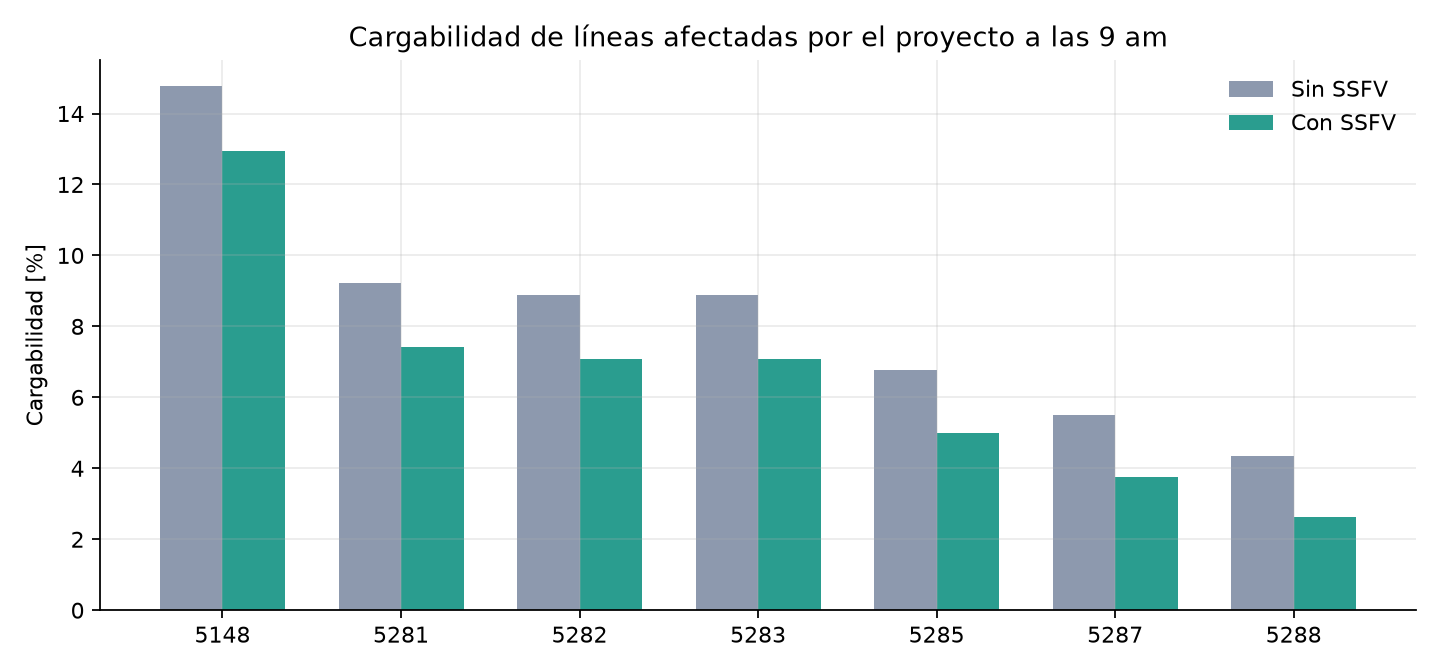
\includegraphics[width=0.95\textwidth]{figuras/fig_cargabilidad_lineas_09.png}
    \caption{Cargabilidad de líneas afectadas por el proyecto Mas X Menos sede Guarín a las 9~am}
    \label{fig:carglineas}
\end{figure}

\begin{table}[H]
    \centering
    \caption{Cargabilidad de líneas a las 9:00 (máxima reducción)}
    \label{tab:carg_lineas}
    \begin{tabular}{lccc}
\toprule
\textbf{Línea} & \textbf{Sin SSFV (\%)} & \textbf{Con SSFV (\%)} & \textbf{Variación (\%)} \\
\midrule
5148 & 14,777 & 12,942 & $-$1,835 \\
5281 & 9,227 & 7,417 & $-$1,810 \\
5282 & 8,884 & 7,077 & $-$1,807 \\
5283 & 8,885 & 7,078 & $-$1,807 \\
5285 & 6,784 & 5,003 & $-$1,782 \\
5287 & 5,498 & 3,746 & $-$1,752 \\
5288 & 4,341 & 2,639 & $-$1,702 \\
\bottomrule
\end{tabular}

\end{table}

No se violan los límites de cargabilidad del SDL de ESSA. En ninguna línea se observa un aumento de loading atribuible a la generación. Las Tablas~\ref{tab:ln_todas_09}, \ref{tab:ln_todas_12} y~\ref{tab:ln_todas_15} listan las 191--195 líneas en servicio, con loading e intensidad sin y con SSFV.

\begingroup
\footnotesize
\setlength{\tabcolsep}{3.5pt}
\begin{longtable}{lccccc}
\caption{Cargabilidad y corriente de todas las líneas a las 9:00 a.m. (sin y con SSFV)} \label{tab:ln_todas_09} \\
\toprule
\textbf{Línea} & \textbf{Loading sin (\%)} & \textbf{Loading con (\%)} & \textbf{$\Delta$ (pp)} & \textbf{$I$ sin (A)} & \textbf{$I$ con (A)} \\
\midrule
\endfirsthead
\caption[]{Cargabilidad y corriente de todas las líneas a las 9:00 a.m. (sin y con SSFV) (cont.)} \\
\toprule
\textbf{Línea} & \textbf{Loading sin (\%)} & \textbf{Loading con (\%)} & \textbf{$\Delta$ (pp)} & \textbf{$I$ sin (A)} & \textbf{$I$ con (A)} \\
\midrule
\endhead
\midrule
\multicolumn{6}{r}{\textit{Continúa en la página siguiente}} \\
\endfoot
\bottomrule
\endlastfoot
5105 & 17,192 & 15,935 & $-$1,257 & 61,03 & 56,57 \\
5106 & 17,192 & 15,936 & $-$1,257 & 61,03 & 56,57 \\
5108 & 17,192 & 15,936 & $-$1,257 & 61,03 & 56,57 \\
5109 & 17,193 & 15,936 & $-$1,256 & 61,03 & 56,57 \\
5110 & 17,193 & 15,936 & $-$1,257 & 61,03 & 56,57 \\
5111 & 17,193 & 15,937 & $-$1,257 & 61,03 & 56,57 \\
5112 & 17,193 & 15,937 & $-$1,257 & 61,04 & 56,58 \\
5113 & 17,194 & 15,937 & $-$1,256 & 61,04 & 56,58 \\
5117 & 17,194 & 15,937 & $-$1,257 & 61,04 & 56,58 \\
5118 & 17,194 & 15,937 & $-$1,256 & 61,04 & 56,58 \\
5120 & 17,194 & 15,938 & $-$1,256 & 61,04 & 56,58 \\
5127 & 15,074 & 13,820 & $-$1,254 & 53,51 & 49,06 \\
5128 & 14,813 & 13,559 & $-$1,254 & 52,59 & 48,13 \\
5129 & 14,465 & 13,211 & $-$1,254 & 51,35 & 46,90 \\
5130 & 14,465 & 13,211 & $-$1,254 & 51,35 & 46,90 \\
5132 & 2,288 & 2,288 & $-$0,000 & 6,29 & 6,29 \\
5136 & 1,105 & 1,105 & $-$0,000 & 3,04 & 3,04 \\
5140 & 12,170 & 10,920 & $-$1,250 & 43,20 & 38,76 \\
5142 & 14,660 & 13,048 & $-$1,612 & 40,32 & 35,88 \\
5143 & 14,323 & 12,712 & $-$1,611 & 39,39 & 34,96 \\
5145 & 0,756 & 0,755 & $-$0,000 & 2,23 & 2,23 \\
5147 & 13,288 & 11,679 & $-$1,609 & 36,54 & 32,12 \\
5148 & 14,777 & 12,942 & $-$1,835 & 35,61 & 31,19 \\
5153 & 12,951 & 11,343 & $-$1,608 & 35,61 & 31,19 \\
5154 & 10,052 & 8,454 & $-$1,598 & 27,64 & 23,25 \\
5156 & 9,174 & 7,581 & $-$1,593 & 25,23 & 20,85 \\
5157 & 8,686 & 7,096 & $-$1,590 & 23,89 & 19,51 \\
5158 & 8,236 & 6,649 & $-$1,587 & 22,65 & 18,28 \\
5280 & 8,086 & 6,500 & $-$1,586 & 22,24 & 17,87 \\
5281 & 9,227 & 7,417 & $-$1,810 & 22,24 & 17,87 \\
5282 & 8,884 & 7,077 & $-$1,807 & 21,41 & 17,06 \\
5283 & 8,885 & 7,078 & $-$1,807 & 21,41 & 17,06 \\
5285 & 6,784 & 5,003 & $-$1,782 & 16,35 & 12,06 \\
5287 & 5,498 & 3,746 & $-$1,752 & 13,25 & 9,03 \\
5288 & 4,341 & 2,639 & $-$1,702 & 10,46 & 6,36 \\
5289 & 4,341 & 2,639 & $-$1,702 & 10,46 & 6,36 \\
5290 & 4,342 & 2,640 & $-$1,702 & 10,46 & 6,36 \\
5291 & 3,827 & 2,164 & $-$1,663 & 9,22 & 5,22 \\
5292 & 3,827 & 2,165 & $-$1,663 & 9,22 & 5,22 \\
5294 & 3,828 & 2,165 & $-$1,662 & 9,22 & 5,22 \\
5295 & 3,828 & 2,166 & $-$1,662 & 9,22 & 5,22 \\
5296 & 3,828 & 2,166 & $-$1,662 & 9,23 & 5,22 \\
5297 & 3,314 & 1,715 & $-$1,599 & 7,99 & 4,13 \\
5298 & 3,315 & 1,715 & $-$1,599 & 7,99 & 4,13 \\
5300 & 2,388 & 1,055 & $-$1,333 & 5,76 & 2,54 \\
5304 & 0,001 & 0,001 & 0,000 & 0,00 & 0,00 \\
5373 & 3,829 & 2,167 & $-$1,662 & 9,23 & 5,22 \\
9137 & 0,299 & 0,299 & 0,000 & 0,46 & 0,46 \\
9138 & 0,299 & 0,299 & 0,000 & 0,46 & 0,46 \\
9139 & 0,000 & 0,000 & 0,000 & 0,00 & 0,00 \\
9140 & 0,000 & 0,000 & 0,000 & 0,00 & 0,00 \\
9141 & 0,299 & 0,299 & 0,000 & 0,46 & 0,46 \\
9142 & 0,299 & 0,299 & 0,000 & 0,46 & 0,46 \\
9143 & 0,599 & 0,599 & $-$0,000 & 0,93 & 0,93 \\
9253 & 0,599 & 0,599 & $-$0,000 & 0,93 & 0,93 \\
9254 & 0,599 & 0,599 & $-$0,000 & 0,93 & 0,93 \\
9256 & 0,599 & 0,599 & $-$0,000 & 0,93 & 0,93 \\
9257 & 0,599 & 0,599 & $-$0,000 & 0,93 & 0,93 \\
9258 & 0,599 & 0,599 & $-$0,000 & 0,93 & 0,93 \\
9264 & 0,399 & 0,399 & 0,000 & 0,62 & 0,62 \\
9265 & 0,399 & 0,399 & 0,000 & 0,62 & 0,62 \\
9266 & 0,399 & 0,399 & 0,000 & 0,62 & 0,62 \\
9267 & 0,399 & 0,399 & 0,000 & 0,62 & 0,62 \\
9268 & 0,399 & 0,399 & 0,000 & 0,62 & 0,62 \\
9274 & 0,599 & 0,599 & $-$0,000 & 0,93 & 0,93 \\
9275 & 0,599 & 0,599 & $-$0,000 & 0,93 & 0,93 \\
9276 & 0,599 & 0,599 & $-$0,000 & 0,93 & 0,93 \\
9277 & 0,599 & 0,599 & $-$0,000 & 0,93 & 0,93 \\
9299 & 1,264 & 1,264 & $-$0,000 & 1,96 & 1,96 \\
9300 & 1,264 & 1,264 & $-$0,000 & 1,96 & 1,96 \\
9301 & 1,264 & 1,264 & $-$0,000 & 1,96 & 1,96 \\
9302 & 0,266 & 0,266 & 0,000 & 0,41 & 0,41 \\
9320 & 0,399 & 0,399 & 0,000 & 0,62 & 0,62 \\
9321 & 0,399 & 0,399 & 0,000 & 0,62 & 0,62 \\
9322 & 0,399 & 0,399 & 0,000 & 0,62 & 0,62 \\
9323 & 0,399 & 0,399 & 0,000 & 0,62 & 0,62 \\
9341 & 0,480 & 0,479 & $-$0,000 & 0,74 & 0,74 \\
9342 & 0,480 & 0,479 & $-$0,000 & 0,74 & 0,74 \\
9344 & 0,959 & 0,959 & $-$0,000 & 1,49 & 1,49 \\
9345 & 0,799 & 0,799 & $-$0,000 & 1,24 & 1,24 \\
9351 & 0,160 & 0,160 & $-$0,000 & 0,25 & 0,25 \\
9352 & 0,160 & 0,160 & $-$0,000 & 0,25 & 0,25 \\
9783 & 0,599 & 0,599 & $-$0,000 & 0,93 & 0,93 \\
9784 & 0,599 & 0,599 & $-$0,000 & 0,93 & 0,93 \\
9785 & 0,599 & 0,599 & $-$0,000 & 0,93 & 0,93 \\
9811 & 0,240 & 0,240 & $-$0,000 & 0,37 & 0,37 \\
9822 & 0,240 & 0,240 & $-$0,000 & 0,37 & 0,37 \\
9823 & 0,240 & 0,240 & $-$0,000 & 0,37 & 0,37 \\
9824 & 0,240 & 0,240 & $-$0,000 & 0,37 & 0,37 \\
9839 & 2,537 & 2,537 & $-$0,000 & 3,93 & 3,93 \\
9840 & 2,605 & 2,604 & $-$0,001 & 4,04 & 4,04 \\
9841 & 2,537 & 2,537 & $-$0,000 & 3,93 & 3,93 \\
9842 & 2,605 & 2,604 & $-$0,001 & 4,04 & 4,04 \\
9843 & 2,664 & 2,664 & $-$0,001 & 4,13 & 4,13 \\
9844 & 2,478 & 2,477 & $-$0,001 & 3,84 & 3,84 \\
9944 & 0,600 & 0,599 & $-$0,000 & 0,93 & 0,93 \\
9945 & 0,600 & 0,599 & $-$0,000 & 0,93 & 0,93 \\
9946 & 0,600 & 0,599 & $-$0,000 & 0,93 & 0,93 \\
9949 & 0,600 & 0,599 & $-$0,000 & 0,93 & 0,93 \\
9950 & 0,600 & 0,599 & $-$0,000 & 0,93 & 0,93 \\
9966 & 0,267 & 0,266 & $-$0,000 & 0,41 & 0,41 \\
9967 & 0,267 & 0,266 & $-$0,000 & 0,41 & 0,41 \\
9989 & 0,799 & 0,799 & $-$0,000 & 1,24 & 1,24 \\
9990 & 0,799 & 0,799 & $-$0,000 & 1,24 & 1,24 \\
9991 & 0,799 & 0,799 & $-$0,000 & 1,24 & 1,24 \\
10833 & 3,266 & 3,265 & $-$0,001 & 5,06 & 5,06 \\
10834 & 1,633 & 1,633 & $-$0,000 & 2,53 & 2,53 \\
10835 & 0,833 & 0,833 & $-$0,000 & 1,29 & 1,29 \\
10836 & 1,067 & 1,066 & $-$0,000 & 1,65 & 1,65 \\
10941 & 0,700 & 0,700 & $-$0,000 & 1,08 & 1,08 \\
10942 & 0,600 & 0,600 & $-$0,000 & 0,93 & 0,93 \\
10943 & 0,600 & 0,600 & $-$0,000 & 0,93 & 0,93 \\
10944 & 0,600 & 0,600 & $-$0,000 & 0,93 & 0,93 \\
10945 & 0,600 & 0,600 & $-$0,000 & 0,93 & 0,93 \\
10978 & 0,700 & 0,700 & $-$0,000 & 1,08 & 1,08 \\
10979 & 0,800 & 0,800 & $-$0,000 & 1,24 & 1,24 \\
11284 & 0,480 & 0,480 & $-$0,000 & 0,74 & 0,74 \\
11285 & 0,520 & 0,520 & $-$0,000 & 0,81 & 0,81 \\
11286 & 0,800 & 0,800 & $-$0,000 & 1,24 & 1,24 \\
11287 & 0,480 & 0,480 & $-$0,000 & 0,74 & 0,74 \\
11288 & 0,400 & 0,400 & $-$0,000 & 0,62 & 0,62 \\
11289 & 0,400 & 0,400 & $-$0,000 & 0,62 & 0,62 \\
11290 & 0,400 & 0,400 & $-$0,000 & 0,62 & 0,62 \\
11342 & 0,400 & 0,400 & $-$0,000 & 0,62 & 0,62 \\
11343 & 0,400 & 0,400 & $-$0,000 & 0,62 & 0,62 \\
11344 & 0,400 & 0,400 & $-$0,000 & 0,62 & 0,62 \\
11381 & 0,400 & 0,400 & $-$0,000 & 0,62 & 0,62 \\
11382 & 0,400 & 0,400 & $-$0,000 & 0,62 & 0,62 \\
11383 & 0,400 & 0,400 & $-$0,000 & 0,62 & 0,62 \\
11384 & 0,400 & 0,400 & $-$0,000 & 0,62 & 0,62 \\
11385 & 0,400 & 0,400 & $-$0,000 & 0,62 & 0,62 \\
15348 & 0,267 & 0,267 & 0,000 & 0,41 & 0,41 \\
15349 & 0,106 & 0,106 & 0,000 & 0,41 & 0,41 \\
15350 & 0,267 & 0,267 & 0,000 & 0,41 & 0,41 \\
15351 & 0,267 & 0,267 & 0,000 & 0,41 & 0,41 \\
21781 & 1,085 & 1,085 & $-$0,000 & 2,17 & 2,17 \\
21782 & 1,085 & 1,085 & $-$0,000 & 2,17 & 2,17 \\
21783 & 0,620 & 0,620 & $-$0,000 & 1,24 & 1,24 \\
26711 & 0,833 & 0,833 & $-$0,000 & 1,29 & 1,29 \\
26712 & 0,600 & 0,600 & $-$0,000 & 0,93 & 0,93 \\
26713 & 0,600 & 0,600 & $-$0,000 & 0,93 & 0,93 \\
40905 & 4,257 & 4,256 & $-$0,000 & 6,60 & 6,60 \\
40906 & 4,257 & 4,256 & $-$0,000 & 6,60 & 6,60 \\
40907 & 4,257 & 4,256 & $-$0,000 & 6,60 & 6,60 \\
47594 & 0,480 & 0,480 & $-$0,000 & 0,74 & 0,74 \\
47595 & 0,520 & 0,520 & $-$0,000 & 0,81 & 0,81 \\
47596 & 0,240 & 0,240 & $-$0,000 & 0,37 & 0,37 \\
47597 & 0,240 & 0,240 & $-$0,000 & 0,37 & 0,37 \\
714206 & 1,563 & 1,562 & $-$0,000 & 2,42 & 2,42 \\
714207 & 1,530 & 1,530 & $-$0,000 & 2,37 & 2,37 \\
714208 & 2,662 & 2,661 & $-$0,000 & 4,13 & 4,13 \\
714209 & 2,662 & 2,661 & $-$0,000 & 4,13 & 4,13 \\
714525 & 0,404 & 0,404 & $-$0,000 & 0,93 & 0,93 \\
717305 & 0,399 & 0,399 & 0,000 & 0,62 & 0,62 \\
717306 & 0,399 & 0,399 & 0,000 & 0,62 & 0,62 \\
720189 & 1,509 & 1,508 & $-$0,000 & 2,34 & 2,34 \\
720190 & 1,509 & 1,508 & $-$0,000 & 2,34 & 2,34 \\
720191 & 1,509 & 1,508 & $-$0,000 & 2,34 & 2,34 \\
720192 & 1,530 & 1,530 & $-$0,000 & 2,37 & 2,37 \\
720193 & 0,399 & 0,399 & 0,000 & 0,62 & 0,62 \\
720194 & 0,399 & 0,399 & 0,000 & 0,62 & 0,62 \\
725649 & 0,599 & 0,599 & $-$0,000 & 0,93 & 0,93 \\
725650 & 0,599 & 0,599 & $-$0,000 & 0,93 & 0,93 \\
725659 & 0,599 & 0,599 & $-$0,000 & 0,93 & 0,93 \\
725660 & 0,599 & 0,599 & $-$0,000 & 0,93 & 0,93 \\
741064 & 1,633 & 1,633 & $-$0,000 & 2,53 & 2,53 \\
764757 & 0,599 & 0,599 & $-$0,000 & 0,93 & 0,93 \\
764758 & 0,599 & 0,599 & $-$0,000 & 0,93 & 0,93 \\
764759 & 0,599 & 0,599 & $-$0,000 & 0,93 & 0,93 \\
764760 & 0,599 & 0,599 & $-$0,000 & 0,93 & 0,93 \\
791042 & 0,400 & 0,400 & $-$0,000 & 0,62 & 0,62 \\
791043 & 0,400 & 0,400 & $-$0,000 & 0,62 & 0,62 \\
791044 & 0,400 & 0,400 & $-$0,000 & 0,62 & 0,62 \\
791045 & 0,400 & 0,400 & $-$0,000 & 0,62 & 0,62 \\
804306 & 15,649 & 14,505 & $-$1,144 & 61,03 & 56,57 \\
806799 & 0,599 & 0,599 & $-$0,000 & 0,93 & 0,93 \\
807671 & 1,915 & 1,731 & $-$0,184 & 2,97 & 2,68 \\
807672 & 1,915 & 1,731 & $-$0,184 & 2,97 & 2,68 \\
807673 & 1,915 & 1,731 & $-$0,184 & 2,97 & 2,68 \\
807674 & 1,915 & 1,731 & $-$0,184 & 2,97 & 2,68 \\
807675 & 1,915 & 1,731 & $-$0,184 & 2,97 & 2,68 \\
812080 & 1,600 & 1,599 & $-$0,001 & 2,48 & 2,48 \\
812081 & 1,600 & 1,599 & $-$0,001 & 2,48 & 2,48 \\
812082 & 1,600 & 1,599 & $-$0,001 & 2,48 & 2,48 \\
812083 & 1,600 & 1,599 & $-$0,001 & 2,48 & 2,48 \\
825166 & 0,533 & 0,533 & $-$0,000 & 0,83 & 0,83 \\
825167 & 0,533 & 0,533 & $-$0,000 & 0,83 & 0,83 \\
828934 & 2,389 & 1,055 & $-$1,333 & 5,76 & 2,54 \\
828942 & 0,385 & 0,385 & $-$0,000 & 0,93 & 0,93 \\
828945 & 0,002 & 0,002 & 0,000 & 0,00 & 0,00 \\
828948 & 0,001 & 0,001 & 0,000 & 0,00 & 0,00 \\
\end{longtable}
\endgroup

\begingroup
\footnotesize
\setlength{\tabcolsep}{3.5pt}
\begin{longtable}{lccccc}
\caption{Cargabilidad y corriente de todas las líneas a las 12:00 p.m. (sin y con SSFV)} \label{tab:ln_todas_12} \\
\toprule
\textbf{Línea} & \textbf{Loading sin (\%)} & \textbf{Loading con (\%)} & \textbf{$\Delta$ (pp)} & \textbf{$I$ sin (A)} & \textbf{$I$ con (A)} \\
\midrule
\endfirsthead
\caption[]{Cargabilidad y corriente de todas las líneas a las 12:00 p.m. (sin y con SSFV) (cont.)} \\
\toprule
\textbf{Línea} & \textbf{Loading sin (\%)} & \textbf{Loading con (\%)} & \textbf{$\Delta$ (pp)} & \textbf{$I$ sin (A)} & \textbf{$I$ con (A)} \\
\midrule
\endhead
\midrule
\multicolumn{6}{r}{\textit{Continúa en la página siguiente}} \\
\endfoot
\bottomrule
\endlastfoot
5105 & 19,836 & 18,572 & $-$1,264 & 70,42 & 65,93 \\
5106 & 19,836 & 18,572 & $-$1,264 & 70,42 & 65,93 \\
5108 & 19,836 & 18,572 & $-$1,264 & 70,42 & 65,93 \\
5109 & 19,836 & 18,573 & $-$1,264 & 70,42 & 65,93 \\
5110 & 19,837 & 18,573 & $-$1,264 & 70,42 & 65,93 \\
5111 & 19,837 & 18,573 & $-$1,264 & 70,42 & 65,93 \\
5112 & 19,837 & 18,573 & $-$1,264 & 70,42 & 65,93 \\
5113 & 19,837 & 18,573 & $-$1,264 & 70,42 & 65,94 \\
5117 & 19,837 & 18,573 & $-$1,264 & 70,42 & 65,94 \\
5118 & 19,837 & 18,574 & $-$1,264 & 70,42 & 65,94 \\
5120 & 19,838 & 18,574 & $-$1,264 & 70,42 & 65,94 \\
5127 & 17,392 & 16,130 & $-$1,262 & 61,74 & 57,26 \\
5128 & 17,091 & 15,829 & $-$1,262 & 60,67 & 56,19 \\
5129 & 16,689 & 15,428 & $-$1,261 & 59,24 & 54,77 \\
5130 & 16,689 & 15,428 & $-$1,261 & 59,25 & 54,77 \\
5132 & 2,639 & 2,639 & $-$0,000 & 7,26 & 7,26 \\
5136 & 1,275 & 1,275 & $-$0,000 & 3,51 & 3,51 \\
5140 & 14,041 & 12,783 & $-$1,258 & 49,85 & 45,38 \\
5142 & 16,915 & 15,292 & $-$1,623 & 46,51 & 42,05 \\
5143 & 16,525 & 14,903 & $-$1,622 & 45,44 & 40,98 \\
5145 & 0,872 & 0,872 & $-$0,000 & 2,57 & 2,57 \\
5147 & 15,331 & 13,710 & $-$1,620 & 42,16 & 37,70 \\
5148 & 17,049 & 15,201 & $-$1,848 & 41,09 & 36,63 \\
5153 & 14,942 & 13,322 & $-$1,620 & 41,09 & 36,63 \\
5154 & 11,597 & 9,986 & $-$1,611 & 31,89 & 27,46 \\
5156 & 10,584 & 8,976 & $-$1,607 & 29,10 & 24,68 \\
5157 & 10,021 & 8,416 & $-$1,605 & 27,56 & 23,14 \\
5158 & 9,501 & 7,899 & $-$1,603 & 26,13 & 21,72 \\
5280 & 9,328 & 7,726 & $-$1,602 & 25,65 & 21,25 \\
5281 & 10,644 & 8,817 & $-$1,828 & 25,65 & 21,25 \\
5282 & 10,249 & 8,424 & $-$1,825 & 24,70 & 20,30 \\
5283 & 10,249 & 8,424 & $-$1,825 & 24,70 & 20,30 \\
5285 & 7,825 & 6,020 & $-$1,805 & 18,86 & 14,51 \\
5287 & 6,341 & 4,558 & $-$1,783 & 15,28 & 10,98 \\
5288 & 5,005 & 3,259 & $-$1,746 & 12,06 & 7,85 \\
5289 & 5,006 & 3,260 & $-$1,746 & 12,06 & 7,86 \\
5290 & 5,006 & 3,260 & $-$1,746 & 12,06 & 7,86 \\
5291 & 4,412 & 2,694 & $-$1,718 & 10,63 & 6,49 \\
5292 & 4,412 & 2,695 & $-$1,718 & 10,63 & 6,49 \\
5294 & 4,413 & 2,695 & $-$1,717 & 10,63 & 6,49 \\
5295 & 4,413 & 2,696 & $-$1,717 & 10,63 & 6,50 \\
5296 & 4,413 & 2,696 & $-$1,717 & 10,64 & 6,50 \\
5297 & 3,820 & 2,147 & $-$1,673 & 9,21 & 5,17 \\
5298 & 3,820 & 2,147 & $-$1,673 & 9,21 & 5,17 \\
5300 & 2,751 & 1,259 & $-$1,492 & 6,63 & 3,03 \\
5304 & 0,001 & 0,001 & 0,000 & 0,00 & 0,00 \\
5373 & 4,414 & 2,697 & $-$1,717 & 10,64 & 6,50 \\
9137 & 0,345 & 0,345 & 0,000 & 0,54 & 0,54 \\
9138 & 0,345 & 0,345 & 0,000 & 0,54 & 0,54 \\
9139 & 0,000 & 0,000 & 0,000 & 0,00 & 0,00 \\
9140 & 0,000 & 0,000 & 0,000 & 0,00 & 0,00 \\
9141 & 0,345 & 0,345 & 0,000 & 0,54 & 0,54 \\
9142 & 0,345 & 0,345 & 0,000 & 0,54 & 0,54 \\
9143 & 0,691 & 0,691 & $-$0,000 & 1,07 & 1,07 \\
9253 & 0,691 & 0,691 & $-$0,000 & 1,07 & 1,07 \\
9254 & 0,691 & 0,691 & $-$0,000 & 1,07 & 1,07 \\
9256 & 0,691 & 0,691 & $-$0,000 & 1,07 & 1,07 \\
9257 & 0,691 & 0,691 & $-$0,000 & 1,07 & 1,07 \\
9258 & 0,691 & 0,691 & $-$0,000 & 1,07 & 1,07 \\
9264 & 0,461 & 0,460 & $-$0,000 & 0,71 & 0,71 \\
9265 & 0,461 & 0,460 & $-$0,000 & 0,71 & 0,71 \\
9266 & 0,461 & 0,460 & $-$0,000 & 0,71 & 0,71 \\
9267 & 0,461 & 0,460 & $-$0,000 & 0,71 & 0,71 \\
9268 & 0,461 & 0,460 & $-$0,000 & 0,71 & 0,71 \\
9274 & 0,691 & 0,691 & $-$0,000 & 1,07 & 1,07 \\
9275 & 0,691 & 0,691 & $-$0,000 & 1,07 & 1,07 \\
9276 & 0,691 & 0,691 & $-$0,000 & 1,07 & 1,07 \\
9277 & 0,691 & 0,691 & $-$0,000 & 1,07 & 1,07 \\
9299 & 1,459 & 1,459 & $-$0,000 & 2,26 & 2,26 \\
9300 & 1,459 & 1,459 & $-$0,000 & 2,26 & 2,26 \\
9301 & 1,459 & 1,459 & $-$0,000 & 2,26 & 2,26 \\
9302 & 0,307 & 0,307 & 0,000 & 0,48 & 0,48 \\
9320 & 0,461 & 0,461 & $-$0,000 & 0,71 & 0,71 \\
9321 & 0,461 & 0,461 & $-$0,000 & 0,71 & 0,71 \\
9322 & 0,461 & 0,461 & $-$0,000 & 0,71 & 0,71 \\
9323 & 0,461 & 0,461 & $-$0,000 & 0,71 & 0,71 \\
9341 & 0,553 & 0,553 & $-$0,000 & 0,86 & 0,86 \\
9342 & 0,553 & 0,553 & $-$0,000 & 0,86 & 0,86 \\
9344 & 1,107 & 1,107 & $-$0,000 & 1,72 & 1,72 \\
9345 & 0,922 & 0,922 & $-$0,000 & 1,43 & 1,43 \\
9351 & 0,184 & 0,184 & $-$0,000 & 0,29 & 0,29 \\
9352 & 0,184 & 0,184 & $-$0,000 & 0,29 & 0,29 \\
9783 & 0,691 & 0,691 & $-$0,000 & 1,07 & 1,07 \\
9784 & 0,691 & 0,691 & $-$0,000 & 1,07 & 1,07 \\
9785 & 0,691 & 0,691 & $-$0,000 & 1,07 & 1,07 \\
9811 & 0,277 & 0,277 & 0,000 & 0,43 & 0,43 \\
9822 & 0,277 & 0,277 & 0,000 & 0,43 & 0,43 \\
9823 & 0,277 & 0,277 & 0,000 & 0,43 & 0,43 \\
9824 & 0,277 & 0,277 & 0,000 & 0,43 & 0,43 \\
9839 & 2,928 & 2,927 & $-$0,001 & 4,54 & 4,54 \\
9840 & 3,006 & 3,005 & $-$0,001 & 4,66 & 4,66 \\
9841 & 2,928 & 2,927 & $-$0,001 & 4,54 & 4,54 \\
9842 & 3,006 & 3,005 & $-$0,001 & 4,66 & 4,66 \\
9843 & 3,075 & 3,074 & $-$0,001 & 4,77 & 4,76 \\
9844 & 2,859 & 2,859 & $-$0,001 & 4,43 & 4,43 \\
9944 & 0,692 & 0,692 & $-$0,000 & 1,07 & 1,07 \\
9945 & 0,692 & 0,692 & $-$0,000 & 1,07 & 1,07 \\
9946 & 0,692 & 0,692 & $-$0,000 & 1,07 & 1,07 \\
9949 & 0,692 & 0,692 & $-$0,000 & 1,07 & 1,07 \\
9950 & 0,692 & 0,692 & $-$0,000 & 1,07 & 1,07 \\
9966 & 0,307 & 0,307 & $-$0,000 & 0,48 & 0,48 \\
9967 & 0,307 & 0,307 & $-$0,000 & 0,48 & 0,48 \\
9989 & 0,923 & 0,922 & $-$0,000 & 1,43 & 1,43 \\
9990 & 0,923 & 0,922 & $-$0,000 & 1,43 & 1,43 \\
9991 & 0,923 & 0,922 & $-$0,000 & 1,43 & 1,43 \\
10833 & 3,769 & 3,768 & $-$0,001 & 5,84 & 5,84 \\
10834 & 1,885 & 1,884 & $-$0,001 & 2,92 & 2,92 \\
10835 & 0,962 & 0,961 & $-$0,000 & 1,49 & 1,49 \\
10836 & 1,231 & 1,230 & $-$0,000 & 1,91 & 1,91 \\
10941 & 0,808 & 0,807 & $-$0,000 & 1,25 & 1,25 \\
10942 & 0,692 & 0,692 & $-$0,000 & 1,07 & 1,07 \\
10943 & 0,692 & 0,692 & $-$0,000 & 1,07 & 1,07 \\
10944 & 0,692 & 0,692 & $-$0,000 & 1,07 & 1,07 \\
10945 & 0,692 & 0,692 & $-$0,000 & 1,07 & 1,07 \\
10978 & 0,808 & 0,807 & $-$0,000 & 1,25 & 1,25 \\
10979 & 0,923 & 0,923 & $-$0,000 & 1,43 & 1,43 \\
11284 & 0,554 & 0,554 & $-$0,000 & 0,86 & 0,86 \\
11285 & 0,600 & 0,600 & $-$0,000 & 0,93 & 0,93 \\
11286 & 0,924 & 0,923 & $-$0,001 & 1,43 & 1,43 \\
11287 & 0,554 & 0,554 & $-$0,000 & 0,86 & 0,86 \\
11288 & 0,462 & 0,462 & $-$0,000 & 0,72 & 0,72 \\
11289 & 0,462 & 0,462 & $-$0,000 & 0,72 & 0,72 \\
11290 & 0,462 & 0,462 & $-$0,000 & 0,72 & 0,72 \\
11342 & 0,462 & 0,462 & $-$0,000 & 0,72 & 0,72 \\
11343 & 0,462 & 0,462 & $-$0,000 & 0,72 & 0,72 \\
11344 & 0,462 & 0,462 & $-$0,000 & 0,72 & 0,72 \\
11381 & 0,462 & 0,462 & $-$0,000 & 0,72 & 0,72 \\
11382 & 0,462 & 0,462 & $-$0,000 & 0,72 & 0,72 \\
11383 & 0,462 & 0,462 & $-$0,000 & 0,72 & 0,72 \\
11384 & 0,462 & 0,462 & $-$0,000 & 0,72 & 0,72 \\
11385 & 0,462 & 0,462 & $-$0,000 & 0,72 & 0,72 \\
15348 & 0,308 & 0,307 & $-$0,000 & 0,48 & 0,48 \\
15349 & 0,122 & 0,122 & 0,000 & 0,48 & 0,48 \\
15350 & 0,308 & 0,307 & $-$0,000 & 0,48 & 0,48 \\
15351 & 0,308 & 0,307 & $-$0,000 & 0,48 & 0,48 \\
21781 & 1,252 & 1,252 & $-$0,000 & 2,50 & 2,50 \\
21782 & 1,252 & 1,252 & $-$0,000 & 2,50 & 2,50 \\
21783 & 0,716 & 0,715 & $-$0,000 & 1,43 & 1,43 \\
26711 & 0,962 & 0,961 & $-$0,000 & 1,49 & 1,49 \\
26712 & 0,692 & 0,692 & $-$0,000 & 1,07 & 1,07 \\
26713 & 0,692 & 0,692 & $-$0,000 & 1,07 & 1,07 \\
40905 & 4,911 & 4,910 & $-$0,001 & 7,61 & 7,61 \\
40906 & 4,911 & 4,910 & $-$0,001 & 7,61 & 7,61 \\
40907 & 4,911 & 4,910 & $-$0,001 & 7,61 & 7,61 \\
47594 & 0,554 & 0,554 & $-$0,000 & 0,86 & 0,86 \\
47595 & 0,600 & 0,600 & $-$0,000 & 0,93 & 0,93 \\
47596 & 0,277 & 0,277 & $-$0,000 & 0,43 & 0,43 \\
47597 & 0,277 & 0,277 & $-$0,000 & 0,43 & 0,43 \\
714206 & 1,803 & 1,803 & $-$0,000 & 2,79 & 2,79 \\
714207 & 1,766 & 1,766 & $-$0,000 & 2,74 & 2,74 \\
714208 & 3,071 & 3,071 & $-$0,000 & 4,76 & 4,76 \\
714209 & 3,071 & 3,071 & $-$0,000 & 4,76 & 4,76 \\
714525 & 0,467 & 0,466 & $-$0,000 & 1,07 & 1,07 \\
717305 & 0,461 & 0,461 & $-$0,000 & 0,71 & 0,71 \\
717306 & 0,461 & 0,461 & $-$0,000 & 0,71 & 0,71 \\
720189 & 1,741 & 1,740 & $-$0,000 & 2,70 & 2,70 \\
720190 & 1,741 & 1,740 & $-$0,000 & 2,70 & 2,70 \\
720191 & 1,741 & 1,740 & $-$0,000 & 2,70 & 2,70 \\
720192 & 1,766 & 1,766 & $-$0,000 & 2,74 & 2,74 \\
720193 & 0,461 & 0,461 & 0,000 & 0,71 & 0,71 \\
720194 & 0,461 & 0,461 & 0,000 & 0,71 & 0,71 \\
725649 & 0,691 & 0,691 & $-$0,000 & 1,07 & 1,07 \\
725650 & 0,691 & 0,691 & $-$0,000 & 1,07 & 1,07 \\
725659 & 0,691 & 0,691 & $-$0,000 & 1,07 & 1,07 \\
725660 & 0,691 & 0,691 & $-$0,000 & 1,07 & 1,07 \\
741064 & 1,885 & 1,884 & $-$0,001 & 2,92 & 2,92 \\
764757 & 0,691 & 0,691 & $-$0,000 & 1,07 & 1,07 \\
764758 & 0,691 & 0,691 & $-$0,000 & 1,07 & 1,07 \\
764759 & 0,691 & 0,691 & $-$0,000 & 1,07 & 1,07 \\
764760 & 0,691 & 0,691 & $-$0,000 & 1,07 & 1,07 \\
791042 & 0,462 & 0,462 & $-$0,000 & 0,72 & 0,72 \\
791043 & 0,462 & 0,462 & $-$0,000 & 0,72 & 0,72 \\
791044 & 0,462 & 0,462 & $-$0,000 & 0,72 & 0,72 \\
791045 & 0,462 & 0,462 & $-$0,000 & 0,72 & 0,72 \\
804306 & 18,055 & 16,905 & $-$1,150 & 70,42 & 65,93 \\
806799 & 0,691 & 0,691 & $-$0,000 & 1,07 & 1,07 \\
807671 & 2,202 & 1,568 & $-$0,634 & 3,41 & 2,43 \\
807672 & 2,202 & 1,568 & $-$0,634 & 3,41 & 2,43 \\
807673 & 2,202 & 1,568 & $-$0,634 & 3,41 & 2,43 \\
807674 & 2,202 & 1,568 & $-$0,634 & 3,41 & 2,43 \\
807675 & 2,202 & 1,568 & $-$0,634 & 3,41 & 2,43 \\
812080 & 1,846 & 1,846 & $-$0,001 & 2,86 & 2,86 \\
812081 & 1,846 & 1,846 & $-$0,001 & 2,86 & 2,86 \\
812082 & 1,846 & 1,846 & $-$0,001 & 2,86 & 2,86 \\
812083 & 1,846 & 1,846 & $-$0,001 & 2,86 & 2,86 \\
825166 & 0,615 & 0,615 & $-$0,000 & 0,95 & 0,95 \\
825167 & 0,615 & 0,615 & $-$0,000 & 0,95 & 0,95 \\
828934 & 2,752 & 1,259 & $-$1,492 & 6,63 & 3,03 \\
828942 & 0,445 & 0,445 & $-$0,000 & 1,07 & 1,07 \\
828945 & 0,002 & 0,002 & 0,000 & 0,00 & 0,00 \\
828948 & 0,001 & 0,001 & 0,000 & 0,00 & 0,00 \\
\end{longtable}
\endgroup

\begingroup
\footnotesize
\setlength{\tabcolsep}{3.5pt}
\begin{longtable}{lccccc}
\caption{Cargabilidad y corriente de todas las líneas a las 15:00 (sin y con SSFV)} \label{tab:ln_todas_15} \\
\toprule
\textbf{Línea} & \textbf{Loading sin (\%)} & \textbf{Loading con (\%)} & \textbf{$\Delta$ (pp)} & \textbf{$I$ sin (A)} & \textbf{$I$ con (A)} \\
\midrule
\endfirsthead
\caption[]{Cargabilidad y corriente de todas las líneas a las 15:00 (sin y con SSFV) (cont.)} \\
\toprule
\textbf{Línea} & \textbf{Loading sin (\%)} & \textbf{Loading con (\%)} & \textbf{$\Delta$ (pp)} & \textbf{$I$ sin (A)} & \textbf{$I$ con (A)} \\
\midrule
\endhead
\midrule
\multicolumn{6}{r}{\textit{Continúa en la página siguiente}} \\
\endfoot
\bottomrule
\endlastfoot
5105 & 19,309 & 18,047 & $-$1,262 & 68,55 & 64,07 \\
5106 & 19,310 & 18,047 & $-$1,262 & 68,55 & 64,07 \\
5108 & 19,310 & 18,047 & $-$1,262 & 68,55 & 64,07 \\
5109 & 19,310 & 18,048 & $-$1,262 & 68,55 & 64,07 \\
5110 & 19,310 & 18,048 & $-$1,262 & 68,55 & 64,07 \\
5111 & 19,310 & 18,048 & $-$1,262 & 68,55 & 64,07 \\
5112 & 19,311 & 18,048 & $-$1,262 & 68,55 & 64,07 \\
5113 & 19,311 & 18,049 & $-$1,262 & 68,55 & 64,07 \\
5117 & 19,311 & 18,049 & $-$1,262 & 68,55 & 64,07 \\
5118 & 19,311 & 18,049 & $-$1,262 & 68,55 & 64,07 \\
5120 & 19,311 & 18,049 & $-$1,262 & 68,55 & 64,07 \\
5127 & 16,931 & 15,671 & $-$1,260 & 60,10 & 55,63 \\
5128 & 16,637 & 15,377 & $-$1,260 & 59,06 & 54,59 \\
5129 & 16,246 & 14,986 & $-$1,260 & 57,67 & 53,20 \\
5130 & 16,246 & 14,987 & $-$1,260 & 57,67 & 53,20 \\
5132 & 2,569 & 2,569 & $-$0,000 & 7,07 & 7,06 \\
5136 & 1,241 & 1,241 & $-$0,000 & 3,41 & 3,41 \\
5140 & 13,669 & 12,412 & $-$1,257 & 48,52 & 44,06 \\
5142 & 16,466 & 14,845 & $-$1,621 & 45,28 & 40,82 \\
5143 & 16,087 & 14,467 & $-$1,620 & 44,24 & 39,78 \\
5145 & 0,849 & 0,849 & $-$0,000 & 2,50 & 2,50 \\
5147 & 14,924 & 13,306 & $-$1,618 & 41,04 & 36,59 \\
5148 & 16,597 & 14,752 & $-$1,845 & 40,00 & 35,55 \\
5153 & 14,546 & 12,928 & $-$1,617 & 40,00 & 35,55 \\
5154 & 11,290 & 9,682 & $-$1,609 & 31,05 & 26,62 \\
5156 & 10,304 & 8,699 & $-$1,605 & 28,33 & 23,92 \\
5157 & 9,756 & 8,154 & $-$1,602 & 26,83 & 22,42 \\
5158 & 9,250 & 7,651 & $-$1,599 & 25,44 & 21,04 \\
5280 & 9,081 & 7,483 & $-$1,598 & 24,97 & 20,58 \\
5281 & 10,363 & 8,539 & $-$1,824 & 24,97 & 20,58 \\
5282 & 9,978 & 8,156 & $-$1,822 & 24,05 & 19,66 \\
5283 & 9,978 & 8,157 & $-$1,821 & 24,05 & 19,66 \\
5285 & 7,619 & 5,818 & $-$1,800 & 18,36 & 14,02 \\
5287 & 6,174 & 4,397 & $-$1,777 & 14,88 & 10,60 \\
5288 & 4,874 & 3,136 & $-$1,738 & 11,75 & 7,56 \\
5289 & 4,874 & 3,137 & $-$1,738 & 11,75 & 7,56 \\
5290 & 4,875 & 3,137 & $-$1,737 & 11,75 & 7,56 \\
5291 & 4,297 & 2,589 & $-$1,708 & 10,36 & 6,24 \\
5292 & 4,297 & 2,589 & $-$1,708 & 10,36 & 6,24 \\
5294 & 4,297 & 2,590 & $-$1,707 & 10,36 & 6,24 \\
5295 & 4,298 & 2,591 & $-$1,707 & 10,36 & 6,24 \\
5296 & 4,298 & 2,591 & $-$1,707 & 10,36 & 6,24 \\
5297 & 3,720 & 2,060 & $-$1,660 & 8,97 & 4,96 \\
5298 & 3,721 & 2,061 & $-$1,660 & 8,97 & 4,97 \\
5300 & 2,680 & 1,215 & $-$1,465 & 6,46 & 2,93 \\
5304 & 0,001 & 0,001 & 0,000 & 0,00 & 0,00 \\
5373 & 4,298 & 2,592 & $-$1,707 & 10,36 & 6,24 \\
9137 & 0,336 & 0,336 & $-$0,000 & 0,52 & 0,52 \\
9138 & 0,336 & 0,336 & $-$0,000 & 0,52 & 0,52 \\
9139 & 0,000 & 0,000 & 0,000 & 0,00 & 0,00 \\
9140 & 0,000 & 0,000 & 0,000 & 0,00 & 0,00 \\
9141 & 0,336 & 0,336 & $-$0,000 & 0,52 & 0,52 \\
9142 & 0,336 & 0,336 & $-$0,000 & 0,52 & 0,52 \\
9143 & 0,672 & 0,672 & 0,000 & 1,04 & 1,04 \\
9253 & 0,672 & 0,672 & 0,000 & 1,04 & 1,04 \\
9254 & 0,672 & 0,672 & 0,000 & 1,04 & 1,04 \\
9256 & 0,672 & 0,672 & 0,000 & 1,04 & 1,04 \\
9257 & 0,672 & 0,672 & 0,000 & 1,04 & 1,04 \\
9258 & 0,672 & 0,672 & 0,000 & 1,04 & 1,04 \\
9264 & 0,448 & 0,448 & 0,000 & 0,69 & 0,69 \\
9265 & 0,448 & 0,448 & 0,000 & 0,69 & 0,69 \\
9266 & 0,448 & 0,448 & 0,000 & 0,69 & 0,69 \\
9267 & 0,448 & 0,448 & 0,000 & 0,69 & 0,69 \\
9268 & 0,448 & 0,448 & 0,000 & 0,69 & 0,69 \\
9274 & 0,673 & 0,673 & $-$0,000 & 1,04 & 1,04 \\
9275 & 0,673 & 0,673 & $-$0,000 & 1,04 & 1,04 \\
9276 & 0,673 & 0,673 & $-$0,000 & 1,04 & 1,04 \\
9277 & 0,673 & 0,673 & $-$0,000 & 1,04 & 1,04 \\
9299 & 1,420 & 1,420 & $-$0,000 & 2,20 & 2,20 \\
9300 & 1,420 & 1,420 & $-$0,000 & 2,20 & 2,20 \\
9301 & 1,420 & 1,420 & $-$0,000 & 2,20 & 2,20 \\
9302 & 0,299 & 0,299 & $-$0,000 & 0,46 & 0,46 \\
9320 & 0,449 & 0,449 & 0,000 & 0,70 & 0,70 \\
9321 & 0,449 & 0,449 & 0,000 & 0,70 & 0,70 \\
9322 & 0,449 & 0,449 & 0,000 & 0,70 & 0,70 \\
9323 & 0,449 & 0,449 & 0,000 & 0,70 & 0,70 \\
9341 & 0,539 & 0,539 & $-$0,000 & 0,83 & 0,83 \\
9342 & 0,539 & 0,539 & $-$0,000 & 0,83 & 0,83 \\
9344 & 1,077 & 1,077 & $-$0,000 & 1,67 & 1,67 \\
9345 & 0,898 & 0,898 & $-$0,000 & 1,39 & 1,39 \\
9351 & 0,180 & 0,179 & $-$0,000 & 0,28 & 0,28 \\
9352 & 0,180 & 0,179 & $-$0,000 & 0,28 & 0,28 \\
9783 & 0,673 & 0,673 & $-$0,000 & 1,04 & 1,04 \\
9784 & 0,673 & 0,673 & $-$0,000 & 1,04 & 1,04 \\
9785 & 0,673 & 0,673 & $-$0,000 & 1,04 & 1,04 \\
9811 & 0,269 & 0,269 & $-$0,000 & 0,42 & 0,42 \\
9822 & 0,269 & 0,269 & $-$0,000 & 0,42 & 0,42 \\
9823 & 0,269 & 0,269 & $-$0,000 & 0,42 & 0,42 \\
9824 & 0,269 & 0,269 & $-$0,000 & 0,42 & 0,42 \\
9839 & 2,850 & 2,849 & $-$0,001 & 4,42 & 4,42 \\
9840 & 2,926 & 2,925 & $-$0,001 & 4,54 & 4,53 \\
9841 & 2,850 & 2,849 & $-$0,001 & 4,42 & 4,42 \\
9842 & 2,926 & 2,925 & $-$0,001 & 4,54 & 4,53 \\
9843 & 2,993 & 2,992 & $-$0,001 & 4,64 & 4,64 \\
9844 & 2,783 & 2,783 & $-$0,001 & 4,31 & 4,31 \\
9944 & 0,673 & 0,673 & $-$0,000 & 1,04 & 1,04 \\
9945 & 0,673 & 0,673 & $-$0,000 & 1,04 & 1,04 \\
9946 & 0,673 & 0,673 & $-$0,000 & 1,04 & 1,04 \\
9949 & 0,673 & 0,673 & $-$0,000 & 1,04 & 1,04 \\
9950 & 0,673 & 0,673 & $-$0,000 & 1,04 & 1,04 \\
9966 & 0,299 & 0,299 & 0,000 & 0,46 & 0,46 \\
9967 & 0,299 & 0,299 & 0,000 & 0,46 & 0,46 \\
9989 & 0,898 & 0,898 & $-$0,000 & 1,39 & 1,39 \\
9990 & 0,898 & 0,898 & $-$0,000 & 1,39 & 1,39 \\
9991 & 0,898 & 0,898 & $-$0,000 & 1,39 & 1,39 \\
10833 & 3,669 & 3,668 & $-$0,001 & 5,69 & 5,69 \\
10834 & 1,835 & 1,834 & $-$0,001 & 2,84 & 2,84 \\
10835 & 0,936 & 0,936 & $-$0,000 & 1,45 & 1,45 \\
10836 & 1,198 & 1,198 & $-$0,000 & 1,86 & 1,86 \\
10941 & 0,786 & 0,786 & $-$0,000 & 1,22 & 1,22 \\
10942 & 0,674 & 0,674 & $-$0,000 & 1,04 & 1,04 \\
10943 & 0,674 & 0,674 & $-$0,000 & 1,04 & 1,04 \\
10944 & 0,674 & 0,674 & $-$0,000 & 1,04 & 1,04 \\
10945 & 0,674 & 0,674 & $-$0,000 & 1,04 & 1,04 \\
10978 & 0,786 & 0,786 & $-$0,000 & 1,22 & 1,22 \\
10979 & 0,899 & 0,898 & $-$0,000 & 1,39 & 1,39 \\
11284 & 0,539 & 0,539 & $-$0,000 & 0,84 & 0,84 \\
11285 & 0,585 & 0,584 & $-$0,000 & 0,91 & 0,91 \\
11286 & 0,899 & 0,899 & $-$0,001 & 1,39 & 1,39 \\
11287 & 0,539 & 0,539 & $-$0,000 & 0,84 & 0,84 \\
11288 & 0,450 & 0,449 & $-$0,000 & 0,70 & 0,70 \\
11289 & 0,450 & 0,449 & $-$0,000 & 0,70 & 0,70 \\
11290 & 0,450 & 0,449 & $-$0,000 & 0,70 & 0,70 \\
11342 & 0,450 & 0,449 & $-$0,000 & 0,70 & 0,70 \\
11343 & 0,450 & 0,449 & $-$0,000 & 0,70 & 0,70 \\
11344 & 0,450 & 0,449 & $-$0,000 & 0,70 & 0,70 \\
11381 & 0,449 & 0,449 & $-$0,000 & 0,70 & 0,70 \\
11382 & 0,449 & 0,449 & $-$0,000 & 0,70 & 0,70 \\
11383 & 0,449 & 0,449 & $-$0,000 & 0,70 & 0,70 \\
11384 & 0,449 & 0,449 & $-$0,000 & 0,70 & 0,70 \\
11385 & 0,449 & 0,449 & $-$0,000 & 0,70 & 0,70 \\
15348 & 0,299 & 0,299 & $-$0,000 & 0,46 & 0,46 \\
15349 & 0,119 & 0,119 & 0,000 & 0,46 & 0,46 \\
15350 & 0,299 & 0,299 & $-$0,000 & 0,46 & 0,46 \\
15351 & 0,299 & 0,299 & $-$0,000 & 0,46 & 0,46 \\
21781 & 1,219 & 1,218 & $-$0,000 & 2,44 & 2,44 \\
21782 & 1,219 & 1,218 & $-$0,000 & 2,44 & 2,44 \\
21783 & 0,696 & 0,696 & $-$0,000 & 1,39 & 1,39 \\
26711 & 0,936 & 0,936 & $-$0,000 & 1,45 & 1,45 \\
26712 & 0,674 & 0,674 & $-$0,000 & 1,04 & 1,04 \\
26713 & 0,674 & 0,674 & $-$0,000 & 1,04 & 1,04 \\
40905 & 4,780 & 4,780 & $-$0,001 & 7,41 & 7,41 \\
40906 & 4,780 & 4,780 & $-$0,001 & 7,41 & 7,41 \\
40907 & 4,780 & 4,780 & $-$0,001 & 7,41 & 7,41 \\
47594 & 0,539 & 0,539 & $-$0,000 & 0,84 & 0,84 \\
47595 & 0,585 & 0,584 & $-$0,000 & 0,91 & 0,91 \\
47596 & 0,270 & 0,270 & $-$0,000 & 0,42 & 0,42 \\
47597 & 0,270 & 0,270 & $-$0,000 & 0,42 & 0,42 \\
714206 & 1,755 & 1,755 & $-$0,000 & 2,72 & 2,72 \\
714207 & 1,719 & 1,719 & $-$0,000 & 2,66 & 2,66 \\
714208 & 2,989 & 2,989 & $-$0,000 & 4,63 & 4,63 \\
714209 & 2,989 & 2,989 & $-$0,000 & 4,63 & 4,63 \\
714525 & 0,454 & 0,454 & $-$0,000 & 1,04 & 1,04 \\
717305 & 0,449 & 0,448 & $-$0,000 & 0,70 & 0,69 \\
717306 & 0,449 & 0,448 & $-$0,000 & 0,70 & 0,69 \\
720189 & 1,694 & 1,694 & $-$0,000 & 2,63 & 2,63 \\
720190 & 1,694 & 1,694 & $-$0,000 & 2,63 & 2,63 \\
720191 & 1,694 & 1,694 & $-$0,000 & 2,63 & 2,63 \\
720192 & 1,719 & 1,719 & $-$0,000 & 2,66 & 2,66 \\
720193 & 0,448 & 0,448 & $-$0,000 & 0,69 & 0,69 \\
720194 & 0,448 & 0,448 & $-$0,000 & 0,69 & 0,69 \\
725649 & 0,673 & 0,673 & $-$0,000 & 1,04 & 1,04 \\
725650 & 0,673 & 0,673 & $-$0,000 & 1,04 & 1,04 \\
725659 & 0,673 & 0,673 & $-$0,000 & 1,04 & 1,04 \\
725660 & 0,673 & 0,673 & $-$0,000 & 1,04 & 1,04 \\
741064 & 1,835 & 1,834 & $-$0,001 & 2,84 & 2,84 \\
764757 & 0,673 & 0,672 & $-$0,000 & 1,04 & 1,04 \\
764758 & 0,673 & 0,672 & $-$0,000 & 1,04 & 1,04 \\
764759 & 0,673 & 0,672 & $-$0,000 & 1,04 & 1,04 \\
764760 & 0,673 & 0,672 & $-$0,000 & 1,04 & 1,04 \\
791042 & 0,450 & 0,449 & $-$0,000 & 0,70 & 0,70 \\
791043 & 0,450 & 0,449 & $-$0,000 & 0,70 & 0,70 \\
791044 & 0,450 & 0,449 & $-$0,000 & 0,70 & 0,70 \\
791045 & 0,450 & 0,449 & $-$0,000 & 0,70 & 0,70 \\
804306 & 17,576 & 16,427 & $-$1,149 & 68,55 & 64,07 \\
806799 & 0,673 & 0,673 & $-$0,000 & 1,04 & 1,04 \\
807671 & 2,144 & 1,598 & $-$0,546 & 3,32 & 2,48 \\
807672 & 2,144 & 1,598 & $-$0,546 & 3,32 & 2,48 \\
807673 & 2,144 & 1,598 & $-$0,546 & 3,32 & 2,48 \\
807674 & 2,144 & 1,598 & $-$0,546 & 3,32 & 2,48 \\
807675 & 2,144 & 1,598 & $-$0,546 & 3,32 & 2,48 \\
812080 & 1,797 & 1,796 & $-$0,001 & 2,79 & 2,78 \\
812081 & 1,797 & 1,796 & $-$0,001 & 2,79 & 2,78 \\
812082 & 1,797 & 1,796 & $-$0,001 & 2,79 & 2,78 \\
812083 & 1,797 & 1,796 & $-$0,001 & 2,79 & 2,78 \\
825166 & 0,599 & 0,599 & $-$0,000 & 0,93 & 0,93 \\
825167 & 0,599 & 0,599 & $-$0,000 & 0,93 & 0,93 \\
828934 & 2,189 & 0,993 & $-$1,197 & 6,46 & 2,93 \\
828942 & 0,354 & 0,354 & $-$0,000 & 1,04 & 1,04 \\
828945 & 0,000 & 0,000 & 0,000 & 0,00 & 0,00 \\
828948 & 0,000 & 0,000 & 0,000 & 0,00 & 0,00 \\
830653 & 0,000 & 0,000 & 0,000 & 0,00 & 0,00 \\
830654 & 0,000 & 0,000 & 0,000 & 0,00 & 0,00 \\
830655 & 0,000 & 0,000 & 0,000 & 0,00 & 0,00 \\
830657 & 0,000 & 0,000 & 0,000 & 0,00 & 0,00 \\
\end{longtable}
\endgroup


\subsection{Cargabilidad de Transformadores}

El transformador de conexión de 150~kVA experimenta un aumento de cargabilidad asociado a la circulación de la potencia generada hacia la red y hacia la carga local. El incremento máximo es de 30,19 puntos porcentuales; aun así, la cargabilidad permanece siempre por debajo del 57\%, como se observa en la Figura~\ref{fig:cargtrafo} y en la Tabla~\ref{tab:carg_trafo}.

\begin{figure}[H]
    \centering
    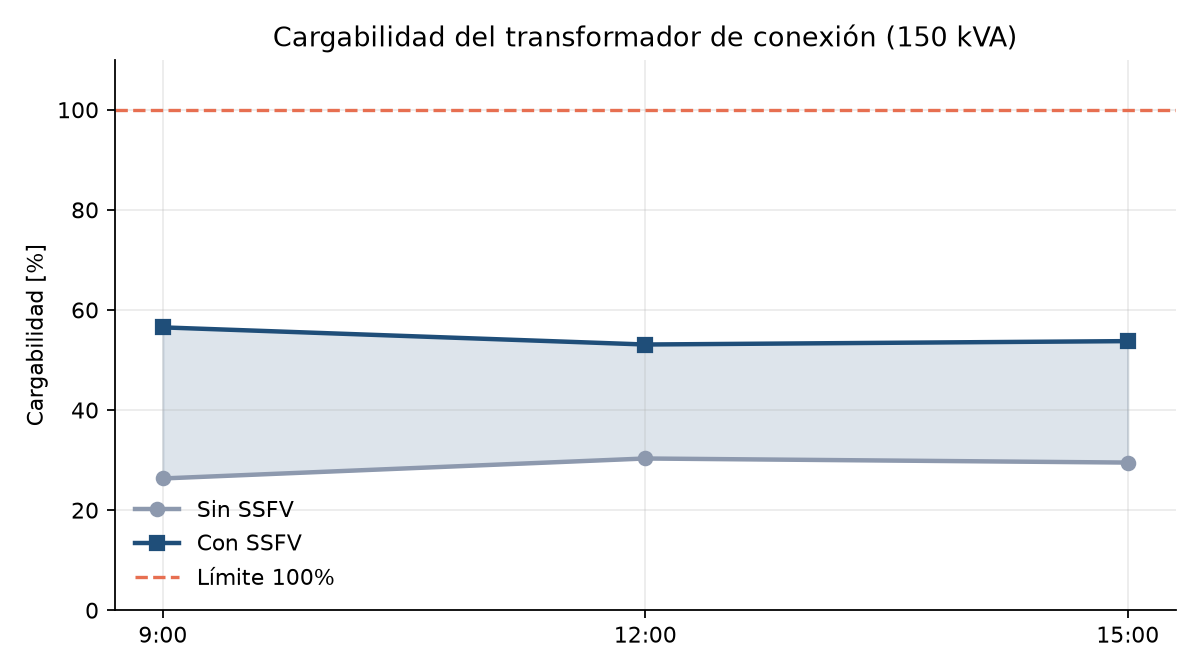
\includegraphics[width=0.90\textwidth]{figuras/fig_cargabilidad_trafo.png}
    \caption{Cargabilidad del transformador de conexión (150 kVA)}
    \label{fig:cargtrafo}
\end{figure}

\begin{table}[H]
    \centering
    \caption{Cargabilidad del transformador de conexión}
    \label{tab:carg_trafo}
    \begin{tabular}{lccc}
\toprule
\textbf{Hora} & \textbf{Sin SSFV (\%)} & \textbf{Con SSFV (\%)} & \textbf{Variación (\%)} \\
\midrule
9:00 a.m. & 26,329 & 56,519 & 30,190 \\
12:00 p.m. & 30,319 & 53,095 & 22,776 \\
15:00 & 29,504 & 53,773 & 24,269 \\
\bottomrule
\end{tabular}

\end{table}

La cargabilidad se mantiene, por tanto, holgadamente bajo el 100\%, con margen suficiente para eventuales crecimientos de demanda o ampliaciones futuras del sistema fotovoltaico dentro de la capacidad del transformador.

\section{Resultados del Estudio de Cortocircuito}

Se calcularon los niveles de cortocircuito trifásico y monofásico en el nodo 3272966 y en nodos aledaños, considerando la entrada en servicio del SSFV de 120~kW. La Figura~\ref{fig:cc} resume los resultados y permite apreciar la similitud entre los escenarios con y sin generación.

\begin{figure}[H]
    \centering
    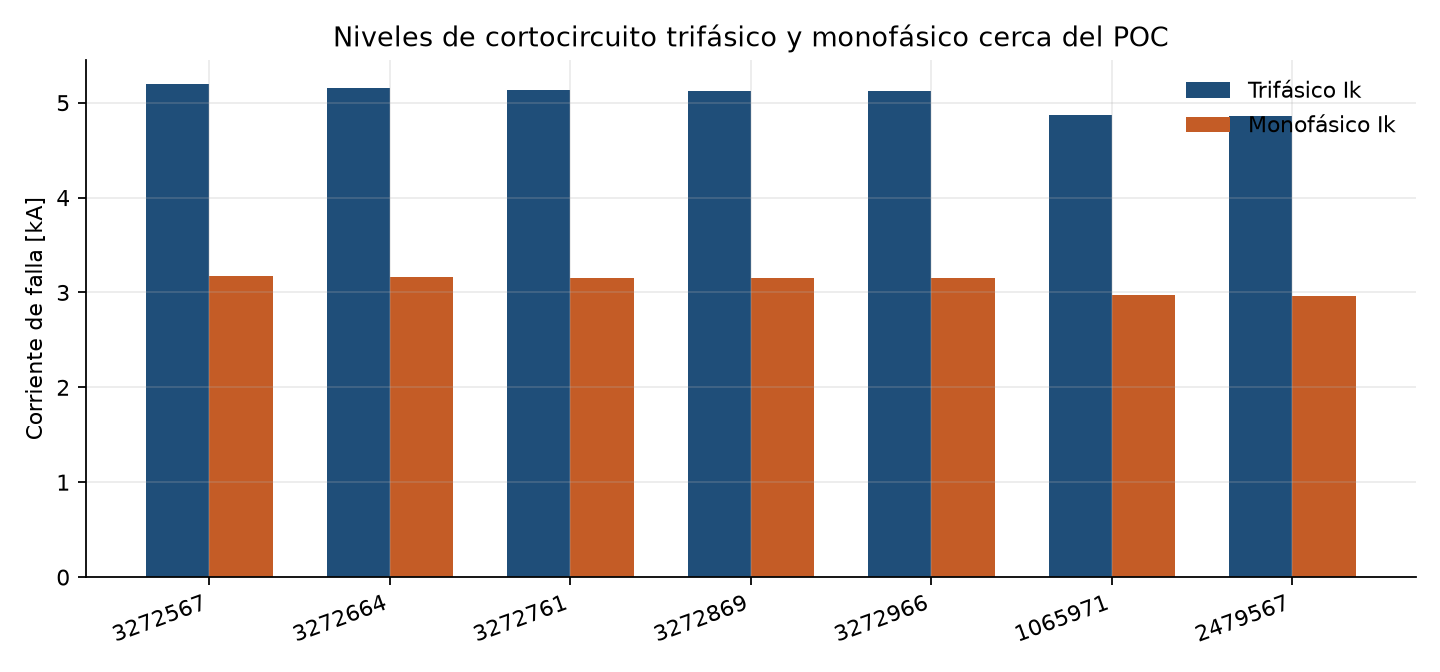
\includegraphics[width=0.95\textwidth]{figuras/fig_cortocircuito.png}
    \caption{Niveles de cortocircuito trifásico y monofásico cerca del POC}
    \label{fig:cc}
\end{figure}

\subsection{Cortocircuito Monofásico}

La Tabla~\ref{tab:cc_1f} presenta las corrientes de falla monofásica a las 12:00 en los nodos de la ruta hacia el POC y en la cabecera del circuito. Las magnitudes se mantienen prácticamente invariantes al incorporar el SSFV, lo que confirma el carácter despreciable del aporte de los inversores en media tensión.

\begin{table}[H]
    \centering
    \caption{Cortocircuito monofásico a las 12:00 (ruta al POC y cabecera)}
    \label{tab:cc_1f}
    \begin{tabular}{lccc}
\toprule
\textbf{Nodo} & \textbf{Sin SSFV (kA)} & \textbf{Con SSFV (kA)} & \textbf{Variación (kA)} \\
\midrule
3272869 & 3,15235 & 3,15235 & 0,00000 \\
3272966 & 3,14984 & 3,14984 & 0,00000 \\
3272761 & 3,15571 & 3,15571 & 0,00000 \\
3272664 & 3,16218 & 3,16218 & 0,00000 \\
3272567 & 3,17766 & 3,17766 & 0,00000 \\
\bottomrule
\end{tabular}

\end{table}

\subsection{Cortocircuito Trifásico}

De manera análoga, la Tabla~\ref{tab:cc_3f} reporta las corrientes de falla trifásica obtenidas con IEC~60909 sobre el equivalente de red. En el POC se obtienen 5,120~kA; en la cabecera del circuito el nivel es de 26,985~kA. La variación de $I_k$ entre escenarios en el bus es nula a la resolución del cálculo, porque el inversor se modela como fuente de corriente (full-size converter) y no entra en la malla de impedancias. El aporte propio se evalúa aparte (Tabla~\ref{tab:cc_aporte}): $1{,}5\,I_L$ referidos a 13,2~kV equivalen a 0,008~kA, el 0,15\% de $I_{k3}$ en el POC, por debajo del 1\%. La Tabla~\ref{tab:cc_todas} reúne $I_{k3}$ e $I_{k1}$ en todos los nodos calculados; la Tabla~\ref{tab:cc_lineas} asigna esas corrientes a los extremos $i$--$j$ de \textbf{todas} las líneas del alimentador. No se requieren modificaciones en las protecciones del circuito 10-502.

\begin{table}[H]
    \centering
    \caption{Cortocircuito trifásico a las 12:00 (ruta al POC y cabecera)}
    \label{tab:cc_3f}
    \begin{tabular}{lccc}
\toprule
\textbf{Nodo} & \textbf{Sin SSFV (kA)} & \textbf{Con SSFV (kA)} & \textbf{Variación (kA)} \\
\midrule
10 502\_Term & 26,98536 & 26,98536 & 0,00000 \\
1067001 & 26,84243 & 26,84243 & 0,00000 \\
3272567 & 5,19351 & 5,19351 & 0,00000 \\
3272664 & 5,15265 & 5,15265 & 0,00000 \\
3272761 & 5,13564 & 5,13564 & 0,00000 \\
3272869 & 5,12685 & 5,12685 & 0,00000 \\
3272966 & 5,12027 & 5,12027 & 0,00000 \\
1065971 & 4,87002 & 4,87002 & 0,00000 \\
2479567 & 4,85776 & 4,85776 & 0,00000 \\
\bottomrule
\end{tabular}

\end{table}

\begin{table}[H]
    \centering
    \caption{Aporte de cortocircuito de los inversores (1,5 $I_L$, referido a MT)}
    \label{tab:cc_aporte}
    \begin{tabular}{lc}
\toprule
\textbf{Magnitud} & \textbf{Valor} \\
\midrule
$I_L$ inversores (220 V) & 314,92 A \\
$I_{k,\mathrm{inv}}$ BT ($1{,}5\,I_L$) & 472,38 A \\
$I_{k,\mathrm{inv}}$ referida a 13,2 kV & 0,00787 kA \\
$I_{k3}$ POC (IEC 60909, red) & 5,12027 kA \\
$I_{k,\mathrm{inv}}/I_{k3}$ POC & 0,15\,\% \\
Criterio de aumento & $< 1$\,\% \\
\bottomrule
\end{tabular}

\end{table}

\begingroup
\footnotesize
\setlength{\tabcolsep}{3.5pt}
\begin{longtable}{lcccccc}
\caption{Cortocircuito IEC~60909 en todos los nodos calculados ($I_{kss}$ en kA, sin y con SSFV)} \label{tab:cc_todas} \\
\toprule
\textbf{Nodo} & \textbf{$I_{k3}$ sin} & \textbf{$I_{k3}$ con} & \textbf{$\Delta_3$} & \textbf{$I_{k1}$ sin} & \textbf{$I_{k1}$ con} & \textbf{$\Delta_1$} \\
\midrule
\endfirsthead
\caption[]{Cortocircuito IEC~60909 en todos los nodos calculados ($I_{kss}$ en kA, sin y con SSFV) (cont.)} \\
\toprule
\textbf{Nodo} & \textbf{$I_{k3}$ sin} & \textbf{$I_{k3}$ con} & \textbf{$\Delta_3$} & \textbf{$I_{k1}$ sin} & \textbf{$I_{k1}$ con} & \textbf{$\Delta_1$} \\
\midrule
\endhead
\midrule
\multicolumn{7}{r}{\textit{Continúa en la página siguiente}} \\
\endfoot
\bottomrule
\endlastfoot
10 502\_Term & 26,98536 & 26,98536 & 0,00000 & 26,96987 & 26,96987 & 0,00000 \\
1067001 & 26,84243 & 26,84243 & 0,00000 & 26,75946 & 26,75946 & 0,00000 \\
3272966 & 5,12027 & 5,12027 & 0,00000 & 3,14984 & 3,14984 & 0,00000 \\
1065971 & 4,87002 & 4,87002 & 0,00000 & 2,97337 & 2,97337 & 0,00000 \\
2479567 & 4,85776 & 4,85776 & 0,00000 & 2,96588 & 2,96588 & 0,00000 \\
3272567 & 5,19351 & 5,19351 & 0,00000 & 3,17766 & 3,17766 & 0,00000 \\
3272664 & 5,15265 & 5,15265 & 0,00000 & 3,16218 & 3,16218 & 0,00000 \\
3272761 & 5,13564 & 5,13564 & 0,00000 & 3,15571 & 3,15571 & 0,00000 \\
3272869 & 5,12685 & 5,12685 & 0,00000 & 3,15235 & 3,15235 & 0,00000 \\
\end{longtable}
\endgroup

\begingroup
\footnotesize
\setlength{\tabcolsep}{3.5pt}
\begin{longtable}{lcccc}
\caption{Corriente de cresta y potencia de cortocircuito en todos los nodos (escenario sin SSFV)} \label{tab:cc_ip_todas} \\
\toprule
\textbf{Nodo} & \textbf{$I_{p3}$ (kA)} & \textbf{$S_{k3}$ (MVA)} & \textbf{$I_{p1}$ (kA)} & \textbf{$S_{k1}$ (MVA)} \\
\midrule
\endfirsthead
\caption[]{Corriente de cresta y potencia de cortocircuito en todos los nodos (escenario sin SSFV) (cont.)} \\
\toprule
\textbf{Nodo} & \textbf{$I_{p3}$ (kA)} & \textbf{$S_{k3}$ (MVA)} & \textbf{$I_{p1}$ (kA)} & \textbf{$S_{k1}$ (MVA)} \\
\midrule
\endhead
\midrule
\multicolumn{5}{r}{\textit{Continúa en la página siguiente}} \\
\endfoot
\bottomrule
\endlastfoot
10 502\_Term & 68,43444 & 645,01 & 68,39520 & 214,88 \\
1067001 & 67,63988 & 641,60 & 67,43082 & 213,20 \\
3272966 & 8,17241 & 122,39 & 5,02742 & 25,10 \\
1065971 & 7,74514 & 116,40 & 4,72876 & 23,69 \\
2479567 & 7,72382 & 116,11 & 4,71573 & 23,63 \\
3272567 & 8,30947 & 124,14 & 5,08417 & 25,32 \\
3272664 & 8,23290 & 123,16 & 5,05253 & 25,19 \\
3272761 & 8,20110 & 122,75 & 5,03935 & 25,14 \\
3272869 & 8,18468 & 122,54 & 5,03252 & 25,12 \\
\end{longtable}
\endgroup

\begingroup
\footnotesize
\setlength{\tabcolsep}{3.5pt}
\begin{longtable}{lcccccc}
\caption{Cortocircuito IEC~60909 en todas las líneas (kA en los nodos extremos $i$ y $j$)} \label{tab:cc_lineas} \\
\toprule
\textbf{Línea} & \textbf{Nodo $i$} & \textbf{Nodo $j$} & \textbf{$I_{k3,i}$} & \textbf{$I_{k3,j}$} & \textbf{$I_{k1,i}$} & \textbf{$I_{k1,j}$} \\
\midrule
\endfirsthead
\caption[]{Cortocircuito IEC~60909 en todas las líneas (kA en los nodos extremos $i$ y $j$) (cont.)} \\
\toprule
\textbf{Línea} & \textbf{Nodo $i$} & \textbf{Nodo $j$} & \textbf{$I_{k3,i}$} & \textbf{$I_{k3,j}$} & \textbf{$I_{k1,i}$} & \textbf{$I_{k1,j}$} \\
\midrule
\endhead
\midrule
\multicolumn{7}{r}{\textit{Continúa en la página siguiente}} \\
\endfoot
\bottomrule
\endlastfoot
5105 & 1067001 & 1069438 & 26,84243 & --- & 26,75946 & --- \\
5106 & 1069438 & 1069446 & --- & --- & --- & --- \\
5108 & 1069446 & 1069454 & --- & --- & --- & --- \\
5109 & 1069454 & 1069471 & --- & --- & --- & --- \\
5110 & 1069471 & 1069489 & --- & --- & --- & --- \\
5111 & 1069489 & 1069497 & --- & --- & --- & --- \\
5112 & 1069497 & 1069501 & --- & --- & --- & --- \\
5113 & 1069501 & 1069519 & --- & --- & --- & --- \\
5117 & 1069519 & 1069527 & --- & --- & --- & --- \\
5118 & 1069527 & 1069683 & --- & --- & --- & --- \\
5120 & 1069683 & 1067010 & --- & --- & --- & --- \\
5127 & 1067010 & 1067028 & --- & --- & --- & --- \\
5128 & 1067036 & 1067028 & --- & --- & --- & --- \\
5129 & 1067036 & 1067044 & --- & --- & --- & --- \\
5130 & 1067044 & 1067052 & --- & --- & --- & --- \\
5132 & 1067052 & 1067079 & --- & --- & --- & --- \\
5136 & 1067079 & 1067087 & --- & --- & --- & --- \\
5140 & 1067052 & 1067109 & --- & --- & --- & --- \\
5142 & 1067109 & 1067117 & --- & --- & --- & --- \\
5143 & 1067117 & 1067125 & --- & --- & --- & --- \\
5145 & 1067125 & 1067133 & --- & --- & --- & --- \\
5147 & 1067125 & 1067141 & --- & --- & --- & --- \\
5148 & 1067141 & 1067150 & --- & --- & --- & --- \\
5153 & 1067150 & 1067176 & --- & --- & --- & --- \\
5154 & 1067176 & 1067184 & --- & --- & --- & --- \\
5156 & 1067184 & 1067192 & --- & --- & --- & --- \\
5157 & 1067192 & 1067206 & --- & --- & --- & --- \\
5158 & 1067206 & 1067214 & --- & --- & --- & --- \\
5280 & 1067214 & 1101251 & --- & --- & --- & --- \\
5281 & 1101251 & 1101277 & --- & --- & --- & --- \\
5282 & 1101277 & 3769721 & --- & --- & --- & --- \\
5283 & 3769721 & 1101293 & --- & --- & --- & --- \\
5285 & 1101293 & 1101307 & --- & --- & --- & --- \\
5287 & 1101307 & 1101315 & --- & --- & --- & --- \\
5288 & 1101315 & 1101323 & --- & --- & --- & --- \\
5289 & 1101323 & 1101331 & --- & --- & --- & --- \\
5290 & 1101331 & 1101340 & --- & --- & --- & --- \\
5291 & 1101340 & 1045288 & --- & --- & --- & --- \\
5292 & 1045288 & 1101358 & --- & --- & --- & --- \\
5294 & 1101358 & 1101374 & --- & --- & --- & --- \\
5295 & 1101374 & 1101382 & --- & --- & --- & --- \\
5296 & 1101382 & 1101391 & --- & --- & --- & --- \\
5297 & 1101404 & 1101412 & --- & --- & --- & --- \\
5298 & 1101412 & 1101421 & --- & --- & --- & --- \\
5300 & 1101421 & 1101447 & --- & --- & --- & --- \\
5304 & 1101480 & 1065971 & --- & 4,87002 & --- & 2,97337 \\
5373 & 1101391 & 1101404 & --- & --- & --- & --- \\
9137 & 1154141 & 1067028 & --- & --- & --- & --- \\
9138 & 1154150 & 1154141 & --- & --- & --- & --- \\
9139 & 1154150 & 1154133 & --- & --- & --- & --- \\
9140 & 1154133 & 1154303 & --- & --- & --- & --- \\
9141 & 1154141 & 1067028 & --- & --- & --- & --- \\
9142 & 1154150 & 1154141 & --- & --- & --- & --- \\
9143 & 1154176 & 1154150 & --- & --- & --- & --- \\
9253 & 1154079 & 1067010 & --- & --- & --- & --- \\
9254 & 1154079 & 1154125 & --- & --- & --- & --- \\
9256 & 1154125 & 1154117 & --- & --- & --- & --- \\
9257 & 1154117 & 1154109 & --- & --- & --- & --- \\
9258 & 1154109 & 1154087 & --- & --- & --- & --- \\
9264 & 1154206 & 1067036 & --- & --- & --- & --- \\
9265 & 1154206 & 1154192 & --- & --- & --- & --- \\
9266 & 1154192 & 1154222 & --- & --- & --- & --- \\
9267 & 1154222 & 1154231 & --- & --- & --- & --- \\
9268 & 1154231 & 1154435 & --- & --- & --- & --- \\
9274 & 1067141 & 1154249 & --- & --- & --- & --- \\
9275 & 1154249 & 1154257 & --- & --- & --- & --- \\
9276 & 1154257 & 1154273 & --- & --- & --- & --- \\
9277 & 1154273 & 1154290 & --- & --- & --- & --- \\
9299 & 1067109 & 1102958 & --- & --- & --- & --- \\
9300 & 1102958 & 1102974 & --- & --- & --- & --- \\
9301 & 1102974 & 1154508 & --- & --- & --- & --- \\
9302 & 1154508 & 1102982 & --- & --- & --- & --- \\
9320 & 1067125 & 1154443 & --- & --- & --- & --- \\
9321 & 1154443 & 1154451 & --- & --- & --- & --- \\
9322 & 1154451 & 1154478 & --- & --- & --- & --- \\
9323 & 1154478 & 1154494 & --- & --- & --- & --- \\
9341 & 1154575 & 1067184 & --- & --- & --- & --- \\
9342 & 1154575 & 1067184 & --- & --- & --- & --- \\
9344 & 1154575 & 1154583 & --- & --- & --- & --- \\
9345 & 1154583 & 1154591 & --- & --- & --- & --- \\
9351 & 1154583 & 1103211 & --- & --- & --- & --- \\
9352 & 1103211 & 1103229 & --- & --- & --- & --- \\
9783 & 1067117 & 1154346 & --- & --- & --- & --- \\
9784 & 1154346 & 1154354 & --- & --- & --- & --- \\
9785 & 1154354 & 1154311 & --- & --- & --- & --- \\
9811 & 1067133 & 1103296 & --- & --- & --- & --- \\
9822 & 1103296 & 1103300 & --- & --- & --- & --- \\
9823 & 1103300 & 1103326 & --- & --- & --- & --- \\
9824 & 1103326 & 1103318 & --- & --- & --- & --- \\
9839 & 1154389 & 1067176 & --- & --- & --- & --- \\
9840 & 1154371 & 1067176 & --- & --- & --- & --- \\
9841 & 1154397 & 1154389 & --- & --- & --- & --- \\
9842 & 1154371 & 1154397 & --- & --- & --- & --- \\
9843 & 1154397 & 1154401 & --- & --- & --- & --- \\
9844 & 1154397 & 1154214 & --- & --- & --- & --- \\
9944 & 1067184 & 1154524 & --- & --- & --- & --- \\
9945 & 1154524 & 1154532 & --- & --- & --- & --- \\
9946 & 1154532 & 1154541 & --- & --- & --- & --- \\
9949 & 1067192 & 1103245 & --- & --- & --- & --- \\
9950 & 1103245 & 1103253 & --- & --- & --- & --- \\
9966 & 1067192 & 1103351 & --- & --- & --- & --- \\
9967 & 1103351 & 1103385 & --- & --- & --- & --- \\
9989 & 1103393 & 1067206 & --- & --- & --- & --- \\
9990 & 1103393 & 1667262 & --- & --- & --- & --- \\
9991 & 1667262 & 1103407 & --- & --- & --- & --- \\
10833 & 1101293 & 1155245 & --- & --- & --- & --- \\
10834 & 1155245 & 1155270 & --- & --- & --- & --- \\
10835 & 1155270 & 1155253 & --- & --- & --- & --- \\
10836 & 1155253 & 1155911 & --- & --- & --- & --- \\
10941 & 1155334 & 1101315 & --- & --- & --- & --- \\
10942 & 1155334 & 1155342 & --- & --- & --- & --- \\
10943 & 1155342 & 1155351 & --- & --- & --- & --- \\
10944 & 1155351 & 1155377 & --- & --- & --- & --- \\
10945 & 1155377 & 1155679 & --- & --- & --- & --- \\
10978 & 1155334 & 1101315 & --- & --- & --- & --- \\
10979 & 1155334 & 1157019 & --- & --- & --- & --- \\
11284 & 1101421 & 1155741 & --- & --- & --- & --- \\
11285 & 1155741 & 1155750 & --- & --- & --- & --- \\
11286 & 1155750 & 1155776 & --- & --- & --- & --- \\
11287 & 1101421 & 1155741 & --- & --- & --- & --- \\
11288 & 1155792 & 1155741 & --- & --- & --- & --- \\
11289 & 1155792 & 1155806 & --- & --- & --- & --- \\
11290 & 1155806 & 1155822 & --- & --- & --- & --- \\
11342 & 1155849 & 1101404 & --- & --- & --- & --- \\
11343 & 1155849 & 1155857 & --- & --- & --- & --- \\
11344 & 1155857 & 1155881 & --- & --- & --- & --- \\
11381 & 1155938 & 1101340 & --- & --- & --- & --- \\
11382 & 1155938 & 1155946 & --- & --- & --- & --- \\
11383 & 1155652 & 1101340 & --- & --- & --- & --- \\
11384 & 1155652 & 1155971 & --- & --- & --- & --- \\
11385 & 1155971 & 1155997 & --- & --- & --- & --- \\
15348 & 1067214 & 1667238 & --- & --- & --- & --- \\
15349 & 1667238 & 1103725 & --- & --- & --- & --- \\
15350 & 1103725 & 1154605 & --- & --- & --- & --- \\
15351 & 1154605 & 1154613 & --- & --- & --- & --- \\
21781 & 1101307 & 2214130 & --- & --- & --- & --- \\
21782 & 2214130 & 2214148 & --- & --- & --- & --- \\
21783 & 2214148 & 2214156 & --- & --- & --- & --- \\
26711 & 1155270 & 1155253 & --- & --- & --- & --- \\
26712 & 1155253 & 2567814 & --- & --- & --- & --- \\
26713 & 2567814 & 2567831 & --- & --- & --- & --- \\
40905 & 1067010 & 2765811 & --- & --- & --- & --- \\
40906 & 2765811 & 2765829 & --- & --- & --- & --- \\
40907 & 2765829 & 2765837 & --- & --- & --- & --- \\
47594 & 1101421 & 1155741 & --- & --- & --- & --- \\
47595 & 1155741 & 1155750 & --- & --- & --- & --- \\
47596 & 1155750 & 2789132 & --- & --- & --- & --- \\
47597 & 2789132 & 2789141 & --- & --- & --- & --- \\
714206 & 1067087 & 4249330 & --- & --- & --- & --- \\
714207 & 4249330 & 4249348 & --- & --- & --- & --- \\
714208 & 4249348 & 4249356 & --- & --- & --- & --- \\
714209 & 4249356 & 4249372 & --- & --- & --- & --- \\
714525 & 2214148 & 4938216 & --- & --- & --- & --- \\
717305 & 1154508 & 1026682 & --- & --- & --- & --- \\
717306 & 1026682 & 1026666 & --- & --- & --- & --- \\
720189 & 1067079 & 5605024 & --- & --- & --- & --- \\
720190 & 5605024 & 5605032 & --- & --- & --- & --- \\
720191 & 5605032 & 4249330 & --- & --- & --- & --- \\
720192 & 4249330 & 4249348 & --- & --- & --- & --- \\
720193 & 4249348 & 1283235 & --- & --- & --- & --- \\
720194 & 1283235 & 5604524 & --- & --- & --- & --- \\
725649 & 8339694 & 8338973 & --- & --- & --- & --- \\
725650 & 8339155 & 8339694 & --- & --- & --- & --- \\
725659 & 8339708 & 8339155 & --- & --- & --- & --- \\
725660 & 1154508 & 8339708 & --- & --- & --- & --- \\
741064 & 1155245 & 1155270 & --- & --- & --- & --- \\
764757 & 1067052 & 9500758 & --- & --- & --- & --- \\
764758 & 9500758 & 9500766 & --- & --- & --- & --- \\
764759 & 9500766 & 9500774 & --- & --- & --- & --- \\
764760 & 9500774 & 8795266 & --- & --- & --- & --- \\
791042 & 1618750 & 1101404 & --- & --- & --- & --- \\
791043 & 1618750 & 1618741 & --- & --- & --- & --- \\
791044 & 1618741 & 1618733 & --- & --- & --- & --- \\
791045 & 1618733 & 9219013 & --- & --- & --- & --- \\
804306 & 10 502\_Term & 1067001 & 26,98536 & 26,84243 & 26,96987 & 26,75946 \\
806799 & 1154290 & 1154281 & --- & --- & --- & --- \\
807671 & 1101455 & 3272567 & --- & 5,19351 & --- & 3,17766 \\
807672 & 3272567 & 3272664 & 5,19351 & 5,15265 & 3,17766 & 3,16218 \\
807673 & 3272664 & 3272761 & 5,15265 & 5,13564 & 3,16218 & 3,15571 \\
807674 & 3272761 & 3272869 & 5,13564 & 5,12685 & 3,15571 & 3,15235 \\
807675 & 3272869 & 3272966 & 5,12685 & 5,12027 & 3,15235 & 3,14984 \\
812080 & 1155270 & 3453561 & --- & --- & --- & --- \\
812081 & 3453561 & 3453464 & --- & --- & --- & --- \\
812082 & 3453464 & 3453367 & --- & --- & --- & --- \\
812083 & 3453367 & 3453260 & --- & --- & --- & --- \\
825166 & 1101277 & 1103431 & --- & --- & --- & --- \\
825167 & 1103431 & 1103458 & --- & --- & --- & --- \\
828934 & 1101447 & 1101455 & --- & --- & --- & --- \\
828942 & 1101471 & 1101455 & --- & --- & --- & --- \\
828945 & 1101471 & 1101480 & --- & --- & --- & --- \\
828948 & 1101480 & 2479567 & --- & 4,85776 & --- & 2,96588 \\
830653 & 1101382 & 4637844 & --- & --- & --- & --- \\
830654 & 4637844 & 4637852 & --- & --- & --- & --- \\
830655 & 4637852 & 4637861 & --- & --- & --- & --- \\
830657 & 4637861 & 4916671A & --- & --- & --- & --- \\
\end{longtable}
\endgroup


\section{Protección en el Punto de Conexión}

Además de verificar el impacto sobre el relé de cabecera, es necesario confirmar que el propio proyecto dispone de las funciones de protección exigidas por la regulación. Esta sección resume la corriente nominal del generador, los requisitos del Acuerdo CNO~1322 y los elementos de interrupción previstos.

\subsection{Corriente Nominal del Generador}

La corriente de carga nominal del sistema en baja tensión se obtiene a partir de la potencia AC y de la tensión de salida de los inversores:

\begin{equation}
I_L = \frac{S}{\sqrt{3}\times V_l} = \frac{120}{\sqrt{3}\times 0{,}22} = 314{,}92~\text{A}
\end{equation}

Este valor sirve de referencia para dimensionar los breakers de inversor y de acometida, así como para referir el aporte de generación a media tensión.

\subsection{Requisitos de Protección (Acuerdo CNO 1322)}

El Acuerdo CNO~1322 establece umbrales y tiempos de operación para las funciones de baja tensión, sobretensión y frecuencia que deben incorporar los generadores conectados al SDL. La Tabla~\ref{tab:cno_req} resume esos requerimientos, y la Tabla~\ref{tab:cno_val} presenta la validación correspondiente al proyecto Guarín. El sistema cumple las funciones ANSI~27, 59 y 81~U/O, así como la protección anti-isla; la función de sobrepotencia adelante (ANSI~32) no aplica a esta configuración. La coordinación con el MICOM~P142 del circuito 10-502 no se ve afectada, como se desarrolla en el capítulo de protecciones.

\begin{table}[H]
    \centering
    \caption{Requerimientos de protección por nivel de tensión}
    \label{tab:cno_req}
    \begin{tabular}{lccc}
    \toprule
    \textbf{Función} & \textbf{Umbral} & \textbf{Tiempo} & \textbf{Unidad} \\
    \midrule
    Baja tensión (ANSI 27) -- Etapa 1 & 0,85 & 2,0 & p.u. / s \\
    Baja tensión (ANSI 27) -- Etapa 2 & 0,50 & 0,2 & p.u. / s \\
    Sobretensión (ANSI 59) -- Etapa 1 & $\geq 1{,}15$ & 2,0 & p.u. / s \\
    Sobretensión (ANSI 59) -- Etapa 2 & $\geq 1{,}20$ & 0,1--0,2 & p.u. / s \\
    Subfrecuencia (ANSI 81U) & 57 & 0,5 & Hz / s \\
    Sobrefrecuencia (ANSI 81O) & 63 & 0,5 & Hz / s \\
    \bottomrule
    \end{tabular}
\end{table}

\begin{table}[H]
    \centering
    \caption{Validación de requisitos de protección}
    \label{tab:cno_val}
    \begin{tabular}{lc}
    \toprule
    \textbf{Requerimiento} & \textbf{Validación} \\
    \midrule
    Baja tensión (ANSI 27) & Cumple \\
    Sobrepotencia adelante (ANSI 32) & No aplica \\
    Sobretensión (ANSI 59) & Cumple \\
    Frecuencia (ANSI 81 U/O) & Cumple \\
    Anti-isla & Cumple \\
    Coordinación con MICOM P142 (CTO 10-502) & Sin afectación \\
    \bottomrule
    \end{tabular}
\end{table}

\subsection{Elemento de Interrupción}

Como elementos de interrupción se contemplan protecciones de inversor en el rango $3\times(140\textrm{--}200)$~A y protección de acometida en el rango $3\times(350\textrm{--}500)$~A. Los tiempos de respuesta de estos dispositivos son coherentes con los criterios de las normas IEC~60909 e IEEE~242, y permiten aislar fallas del lado de baja tensión sin comprometer la selectividad respecto al relé de cabecera.

\section{Cálculo de Pérdidas}

La generación distribuida tiende a reducir las pérdidas técnicas del alimentador cuando la energía se consume cerca del punto de inyección. La Figura~\ref{fig:perdidas} y la Tabla~\ref{tab:perdidas} cuantifican ese efecto para las tres franjas de análisis.

\begin{figure}[H]
    \centering
    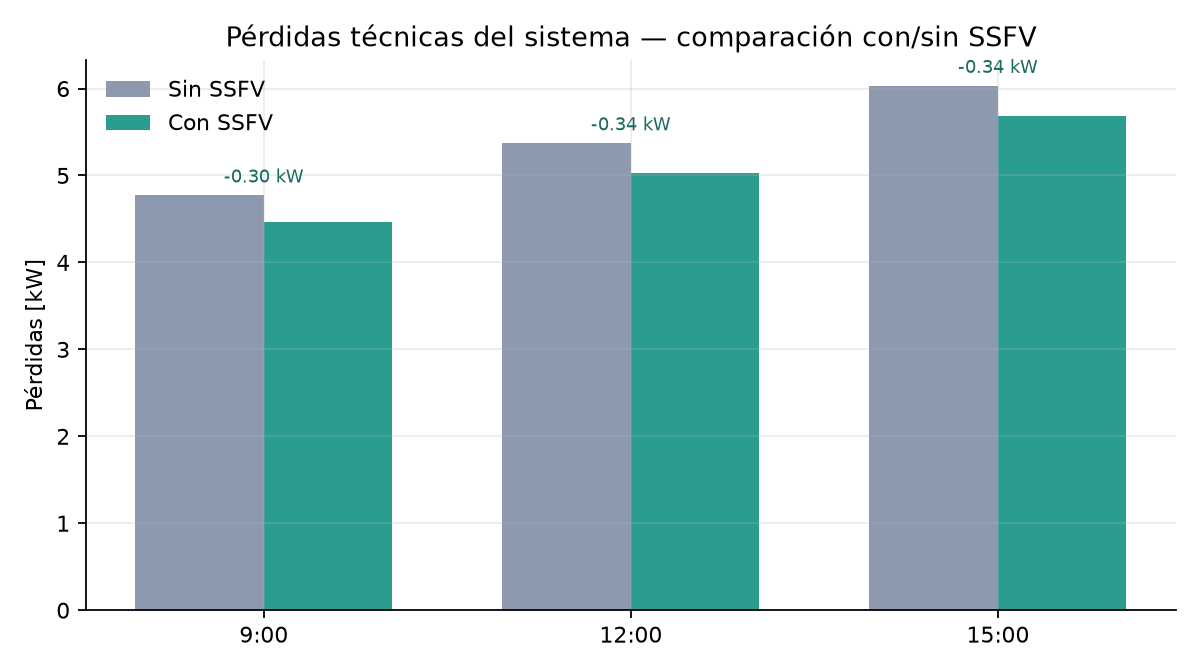
\includegraphics[width=0.90\textwidth]{figuras/fig_perdidas.png}
    \caption{Pérdidas técnicas del sistema con y sin SSFV}
    \label{fig:perdidas}
\end{figure}

\begin{table}[H]
    \centering
    \caption{Pérdidas totales del sistema}
    \label{tab:perdidas}
    \begin{tabular}{lccc}
\toprule
\textbf{Hora} & \textbf{Con SSFV (kW)} & \textbf{Sin SSFV (kW)} & \textbf{Reducción (kW)} \\
\midrule
9:00 a.m. & 3,77 & 3,88 & 0,11 \\
12:00 p.m. & 4,62 & 4,96 & 0,34 \\
15:00 & 4,44 & 4,73 & 0,30 \\
\bottomrule
\end{tabular}

\end{table}

En las tres franjas evaluadas, por tanto, la generación distribuida contribuye a disminuir las pérdidas técnicas del alimentador, lo cual constituye un beneficio adicional de la conexión para el sistema de distribución.

\subsection{Pérdidas Consideradas en Energía Generada}

Para la estimación de energía anual se adoptó un factor global de pérdidas del 26\%, desglosado en la Tabla~\ref{tab:perdidas_fv}. Este desglose incluye temperatura, mismatch, pérdidas resistivas, conversión DC/AC y otras pérdidas asociadas; las pérdidas por sombreado se consideran nulas, en coherencia con la evaluación del sitio.

\begin{table}[H]
    \centering
    \caption{Desglose de pérdidas del sistema fotovoltaico}
    \label{tab:perdidas_fv}
    \begin{tabular}{lc}
    \toprule
    \textbf{Tipo de pérdida} & \textbf{Porcentaje} \\
    \midrule
    Pérdidas por temperatura & 3,00\% \\
    Pérdidas por mismatch & 2,00\% \\
    Pérdidas resistivas & 4,00\% \\
    Pérdidas por conversión DC/AC & 1,00\% \\
    Otras pérdidas asociadas & 16,00\% \\
    Pérdidas por sombreado & 0,00\% \\
    \midrule
    \textbf{Total} & \textbf{26,00\%} \\
    \bottomrule
    \end{tabular}
\end{table}
